% ===================================================================================================
%                                                 |                                                 |
%                                                 |                                                 |
% -------------------------------------------- SECTION ---------------------------------------------|
%                                                 |                                                 |
%                                                 |                                                 |
% ===================================================================================================
\section{Mathematical framework}\label{sec:transfer_learning}
In this section, the goal is to model the demand scaling of energy and time that results from the use of a large number of robots performing a large number of skills.

% ===================================================================================================
\subsection{Energy and time demand for learning skills}
% ---
\begin{figure}[!ht]
	\centering
	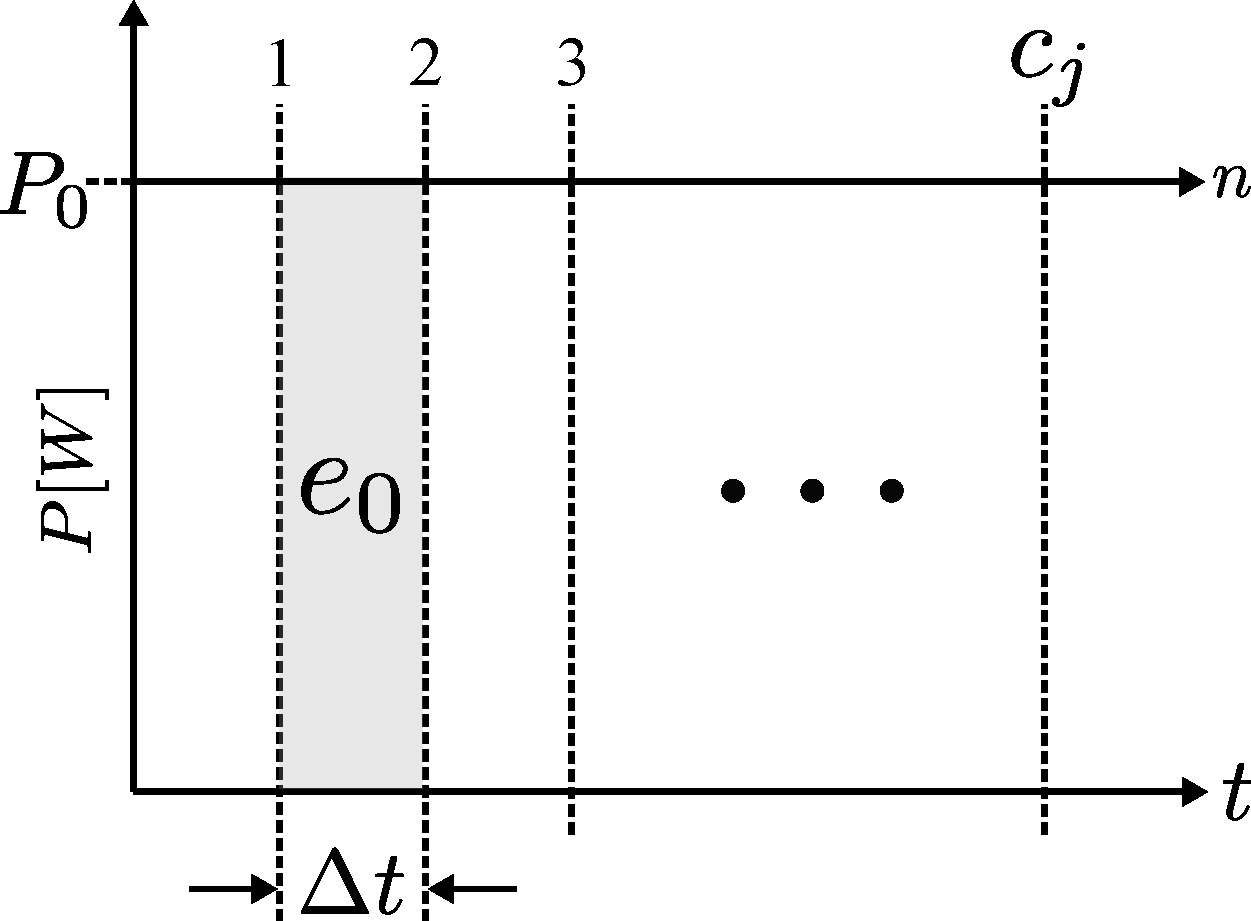
\includegraphics[width=0.9\columnwidth]{fig/power_per_episode.pdf}
	\caption{Power consumption per episode.}
	\label{fig:power_per_episode}
\end{figure}
%---
\begin{tcolorbox}
\begin{definition}\label{definition:complexity} The complexity $c_j$ of a skill $ s_j $  is understood as the number of trial episodes $n$ needed to successfully learn the skill; i.e., all actions and states visited until a stopping criterion is reached. 
\end{definition}
\end{tcolorbox}
% ---
Now, let $P_0$ be the total power\footnote{$P_0$ is assumed to be constant.} required by the robot to sustain the learning. Furthermore,
% ---
\begin{tcolorbox}
\begin{assumption}\label{assumption:time} Every trial episode $n$ takes the same amount of time $\Delta t$ to be executed (Fig.~\ref{fig:power_per_episode}).
\end{assumption}
\end{tcolorbox}
% ---
% ---------------------------------------------------------------------------------------------------
\subsubsection{\textbf{Energy requirement}}
Under Assumption \ref{assumption:time}, the energy consumption of the $n$-th episode $e^{(n)}_j$ is simply
% ---
\begin{equation}\label{eq:energy_per_episode}
    e^{(n)}_j = \cancelto{\text{const}}{P_0\cdot \Delta t} = e_0
\end{equation}
% ---
Consequently, the energy consumed by a robot learning the skill $ s_j $ is directly proportional to the complexity; i.e.
% ---
\begin{equation}\label{eq:energy_per_skill}
    E_j =\sum_{n=1}^{c_j} e^{(n)}_j = e_0 \cdot c_j.
\end{equation}
% ---
Having $\mathcal{S}$ represent the set of all \emph{to-be-learned} skills, with $|\mathcal{S}| = N_\mathcal{S}$; then, the energy spent on learning $\mathcal{S}$ is
% ---
\begin{equation}\label{eq:total_energy}
	E_{\mathcal{S}} = \sum_{j=1}^{{N_{\mathcal{S}}}} E_j = e_0 \sum_{j=1}^{{N_{\mathcal{S}}}} c_j%N_{\mathcal{T}} \cdot e_0 \cdot c_j 
\end{equation}
% ---
%\begin{equation}\label{eq:energy_per_task}
%	E_j =m \sum_{n=1}^{c_j} e^{(n)}_j = m \cdot e_0 \cdot c_j,
%\end{equation}
%\begin{equation}\label{eq:total_energy}
%	E_{\mathcal{S}} = \sum_{j=1}^{{N_{\mathcal{S}}}/{m}} E_j = m \cdot e_0 \sum_{j=1}^{{N_{\mathcal{S}}}/{m}} c_j%N_{\mathcal{T}} \cdot e_0 \cdot c_j 
%\end{equation}
% ---------------------------------------------------------------------------------------------------
\subsubsection{\textbf{Time requirement}}
Similarly, the total time $T_{\mathcal{S}}$ is simply
% ---
\begin{equation}\label{eq:total_energy}
	T_{\mathcal{S}} = \Delta t \sum_{j=1}^{{N_{\mathcal{S}}}} c_j.
\end{equation}
% ---
% ===================================================================================================
\subsection{Skill knowledge}
Consider a knowledge function $\bar{\sigma}_j(\mathcal{Z})\in [0,1]$ that expresses the knowledge from a skill  $s_j \in \mathcal{S}$ that \textbf{is not} contained in a set of already learned skills $\mathcal{Z} \subset \mathcal{S}$; i.e. $s_j \notin \mathcal{Z}$. The function $\bar{\sigma}_j(\cdot)$ satisfies:
\begin{itemize}
	\item $\bar{\sigma}_j(\mathcal{Z}) = 1$, if $\mathcal{Z}=\emptyset$ or if it does not contain knowledge about the skill $s_j$
	\item $\bar{\sigma}_j(\mathcal{Z}) = 0$, if all the knowledge about skill $s_j$ is contained in $\mathcal{Z}$
\end{itemize} 
Conceptually, $\bar{\sigma}_j(\mathcal{Z})$ is the fraction of knowledge that remains to be learned.
% ---------------------------------------------------------------------------------------------------
\subsubsection{\textbf{Leveraging the acquired knowledge}}
To simplify the analysis, we introduce a fundamental complexity
\begin{tcolorbox}
\begin{assumption}\label{definition:joint_grouping} The fundamental complexity $c_0$ describes the maximum number of episodes required to learn \emph{any} skill.
\end{assumption}
\end{tcolorbox}
% ---
If, in learning a skill $ s_j $, a robot uses the knowledge contained in $\mathcal{Z}$ about $s_j$; then, its associated complexity $ c_j $ is a scaled down verison of the complexity $c_{0}$ and is given by:
% ---
\begin{equation}\label{eq:scaled_complexity}
c_j = c_{0} \cdot \bar{\sigma}_{j}\left(\mathcal{Z}\right)\in [0, c_{0}].
\end{equation}
%---
\begin{tcolorbox}
	\begin{assumption}\label{assumption:skill_complexity}
		The skills in $ \mathcal{S} $ share a high degree of similarity (have the same complexity).
	\end{assumption}
\end{tcolorbox}
% ---
Assumption~\ref{assumption:skill_complexity} implies that a new skill $s_j \in \mathcal{S}$ can always benefit from the knowledge contained in $\mathcal{Z} \subset \mathcal{S}$. This implies that the more skills enter $\mathcal{Z}$ (with $|\mathcal{Z}| = N_j$), the less knowledge about $ s_j $ will remain to be learned. Thus, according to \eqref{eq:scaled_complexity} the complexity scales down as a function of the number of learned skills, as exemplified in Fig.~\ref{fig:complexity_per_cardinality}. Alternatively,
% ---
\begin{equation}\label{eq:knowledge_limit}
    \lim_{N_{j}\to N_{\mathcal{S}}} \bar{\sigma}_j = 0 \implies \lim_{N_{j}\to N_{\mathcal{S}}} c_j = 0.
\end{equation}
%---
\begin{figure}[!ht]
	\centering
	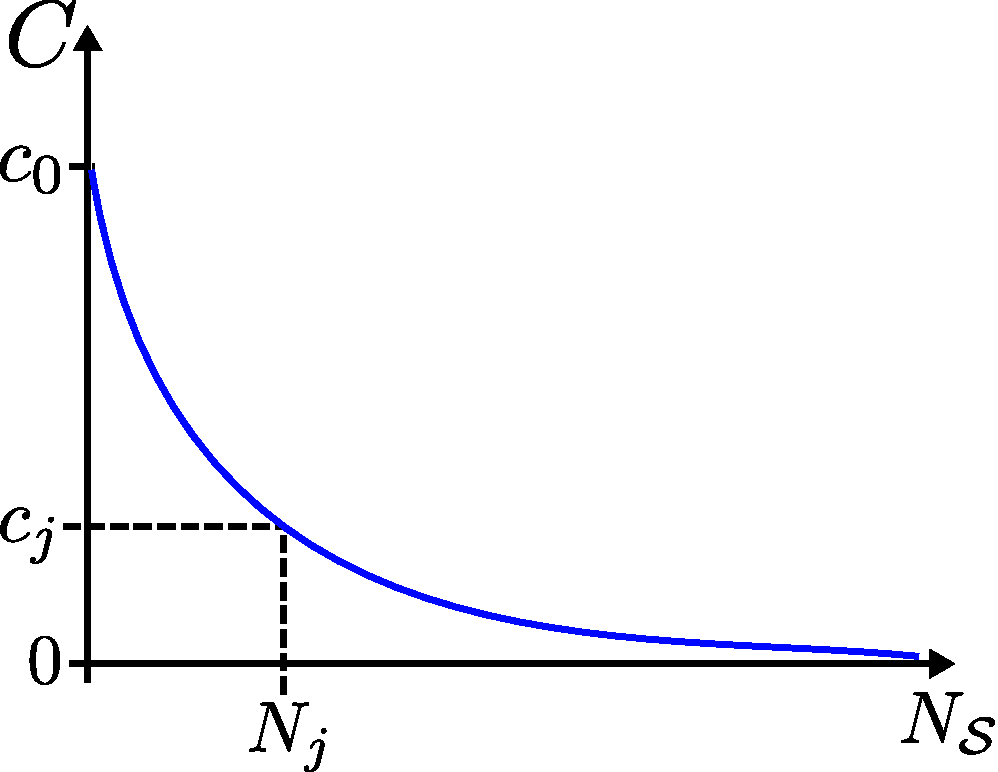
\includegraphics[width=0.7\columnwidth]{fig/complexity_per_cardinality.pdf}
	\caption{The complexity of a skill $c_j$ (number of trial episodes) decreases exponentially with the number of learned skills $|\mathcal{Z}|=N_{j}$.}
	\label{fig:complexity_per_cardinality}
\end{figure}
% ---
%Furthermore, consider the following assumptions
%% ---
%\begin{tcolorbox}
%	\begin{assumption}\label{assumption:skill_clustering} When the degree of similarity among a set of skills is comparable, they can be clustered together.
%	\end{assumption}
%\end{tcolorbox}
%% --- 
%The previous assumption is depicted in Fig.~\ref{fig:incremental_transfer_similarity} where similar skills are grouped together in four different clusters.
\begin{tcolorbox}
	\begin{assumption}\label{assumption:exponential_decrease} The knowledge function $\bar{\sigma}(\cdot)$ has an exponentially decreasing behavior.
	\end{assumption}
\end{tcolorbox} 
% ---
Considering Assumption~\ref{assumption:exponential_decrease}, an idealization of the behavior described by \eqref{eq:knowledge_limit} can be modeled as a decreasing exponential, which is a function of the number of already learned skills $N_j$:% from the cluster $k$; i.e. ${^kN_j}$:
% ---
\begin{equation}\label{eq:incremental_knowledge}
  \bar{\sigma}_j = e^{-\alpha  \cdot N_{j}} \in (0,1],
\end{equation}
% ---
where $ 0<\alpha<<1$ models how effectively the knowledge contained in $\mathcal{Z}$ is shared with $s_j$.

% ===================================================================================================
\subsection{Knowledge sharing under different learning paradigms}
The following assumptions are analogous to average behavior and imply that a suitable scaling strategy is available and executed.
% ---
\begin{tcolorbox}
	\begin{assumption}\label{assumption:agent_similarity}
		Every agent has the same abilities and energetic cost.
	\end{assumption}
\end{tcolorbox}
%---
\begin{tcolorbox}
	\begin{assumption}\label{assumption:skill_clustering} When the degree of similarity among a set of skills is comparable, they can be clustered together.
		\end{assumption}
\end{tcolorbox}
% ---
\begin{tcolorbox}
	\begin{assumption}\label{assumption:cluster_size}
		Every cluster contains the same number of skills.
	\end{assumption}
\end{tcolorbox}
% ---
\begin{tcolorbox}
	\begin{assumption}\label{assumption:cluster_transferability}
		The knowledge transferability between skills is assumed to be equal, therefore, also the transferability between clusters is assumed to be equal.
	\end{assumption}
\end{tcolorbox}
% ---------------------------------------------------------------------------------------------------
\subsubsection{\textbf{Isolated learning (Iso)}} a robot learns all the skills in $\mathcal{S}$ one after another from scratch, disregarding the knowledge from all other learned skills in $\mathcal{Z}$ when learning a new skill. In other words, this implies that $N_j = 0$ in \eqref{eq:incremental_knowledge}. The energy required by the robot to learn all skills in $\mathcal{S}$ is simply
% ---
\begin{align}
    \begin{split}
      E^{(Iso)}_{\mathcal{S}} &= N_{\mathcal{S}} \cdot E^{(Iso)}_j\\ 
      &= N_{\mathcal{S}} \cdot e_{0} \cdot \cancelto{c_{0}}{c_{j}} 
    \end{split}
\end{align}
% ---
Furthermore, using batches of $m$ robots to learning $m$ skills in parallel, needs $m\cdot E^{(Iso)}_j$ \unit[]{J}. Therefore, there are no energy reductions under this scheme.
% ---
\begin{figure}[!t]
	\centering
	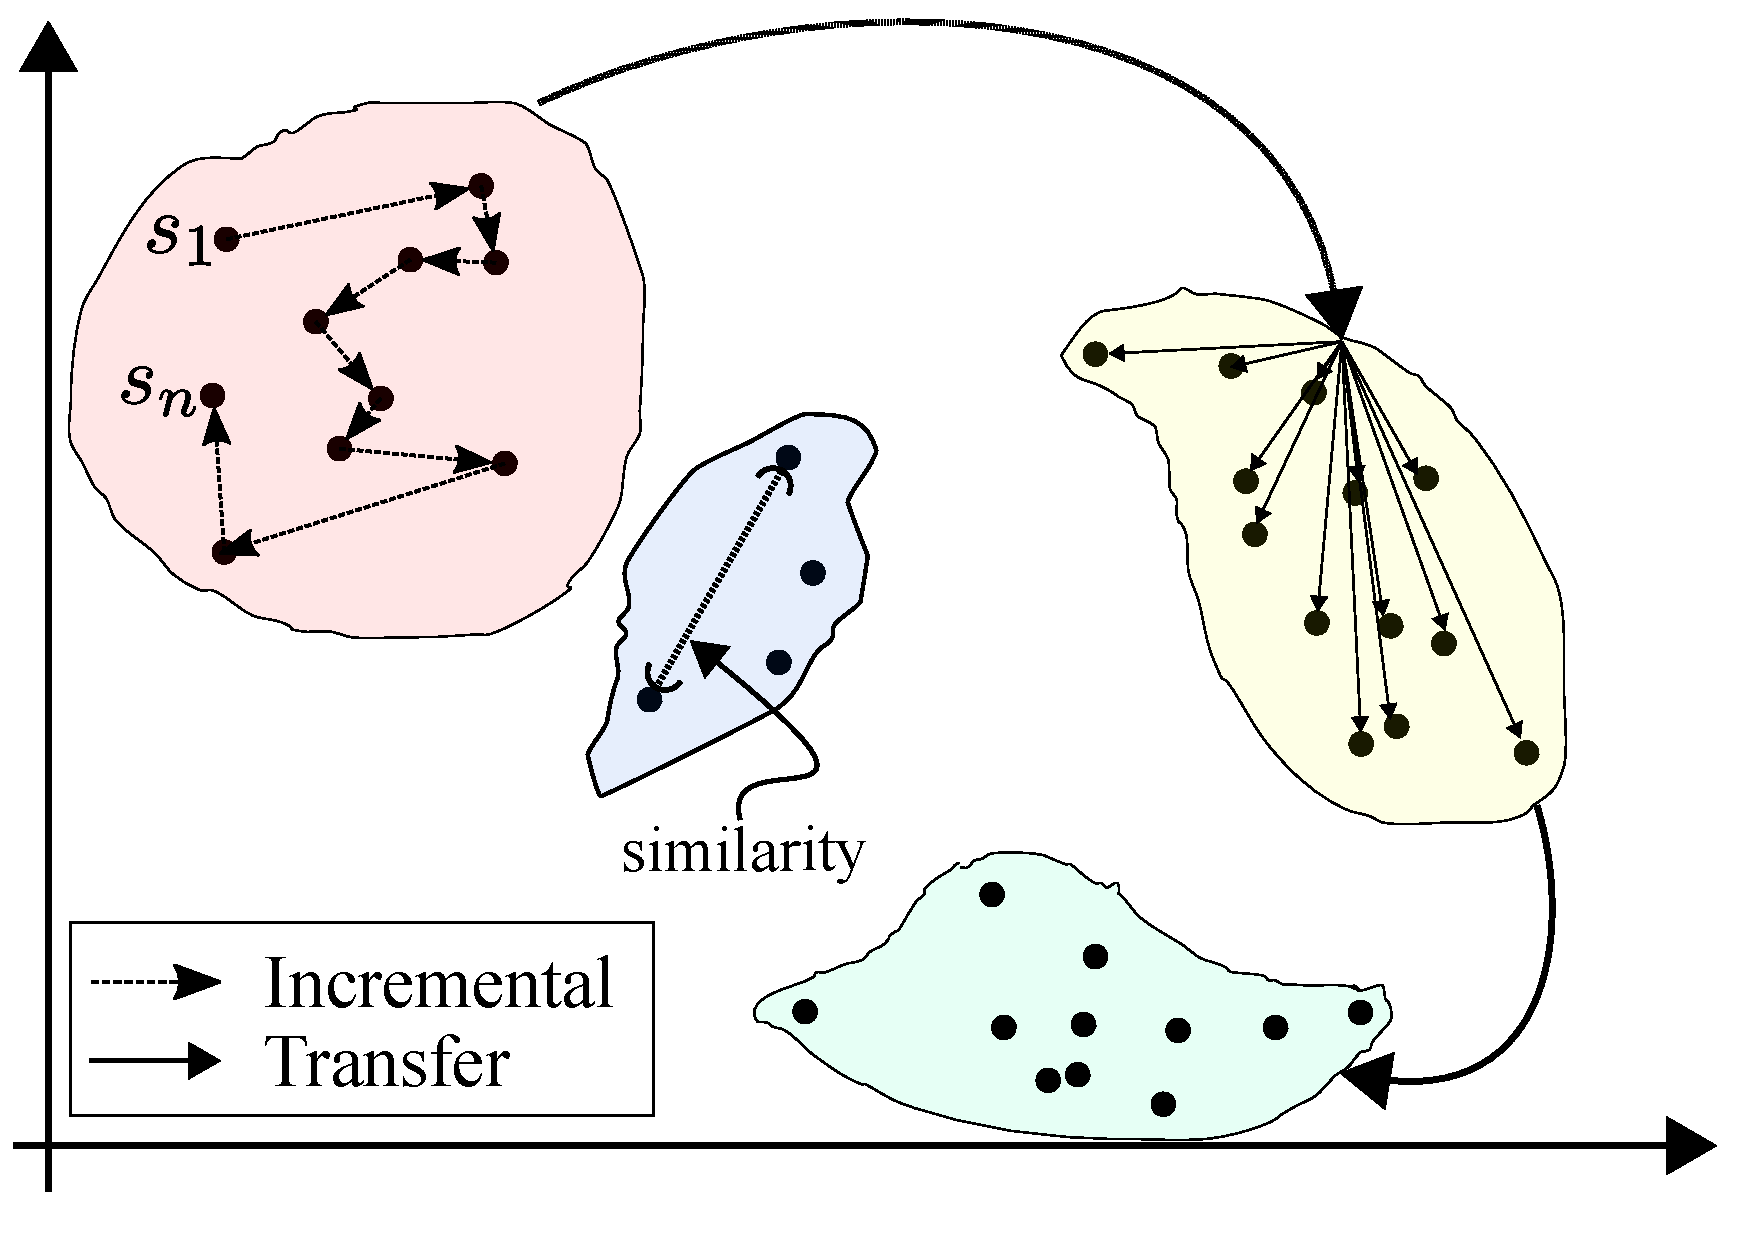
\includegraphics[width=0.9\columnwidth]{fig/incremental_transfer_similarity_v2.pdf}
	\caption{Incremental and transfer learning and its relation to similarity.}
	\label{fig:incremental_transfer_similarity}
\end{figure}
% ---
\begin{figure*}[!htb]
	\centering
	\hspace*{\fill}
	\subfloat[]{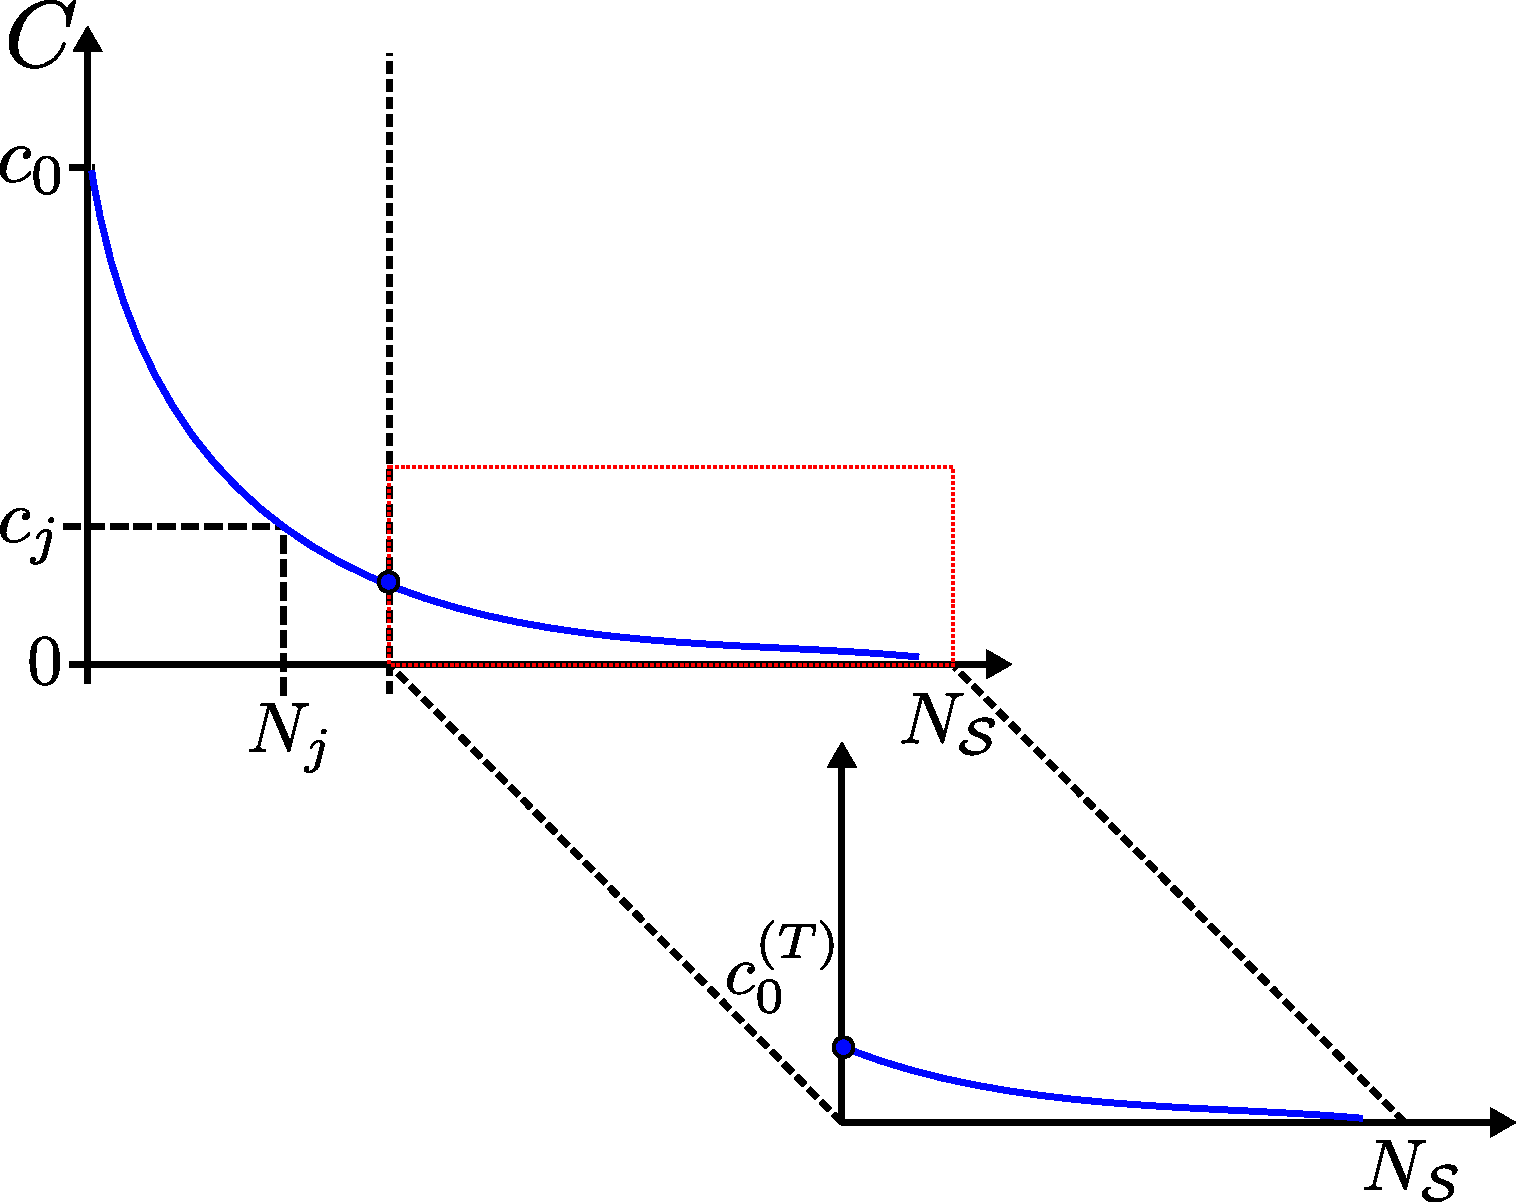
\includegraphics[width= 0.80\columnwidth]{fig/effect_transfer_learning.pdf} \label{fig:effect_transfer_learning}}  
	\hfill
	\subfloat[]{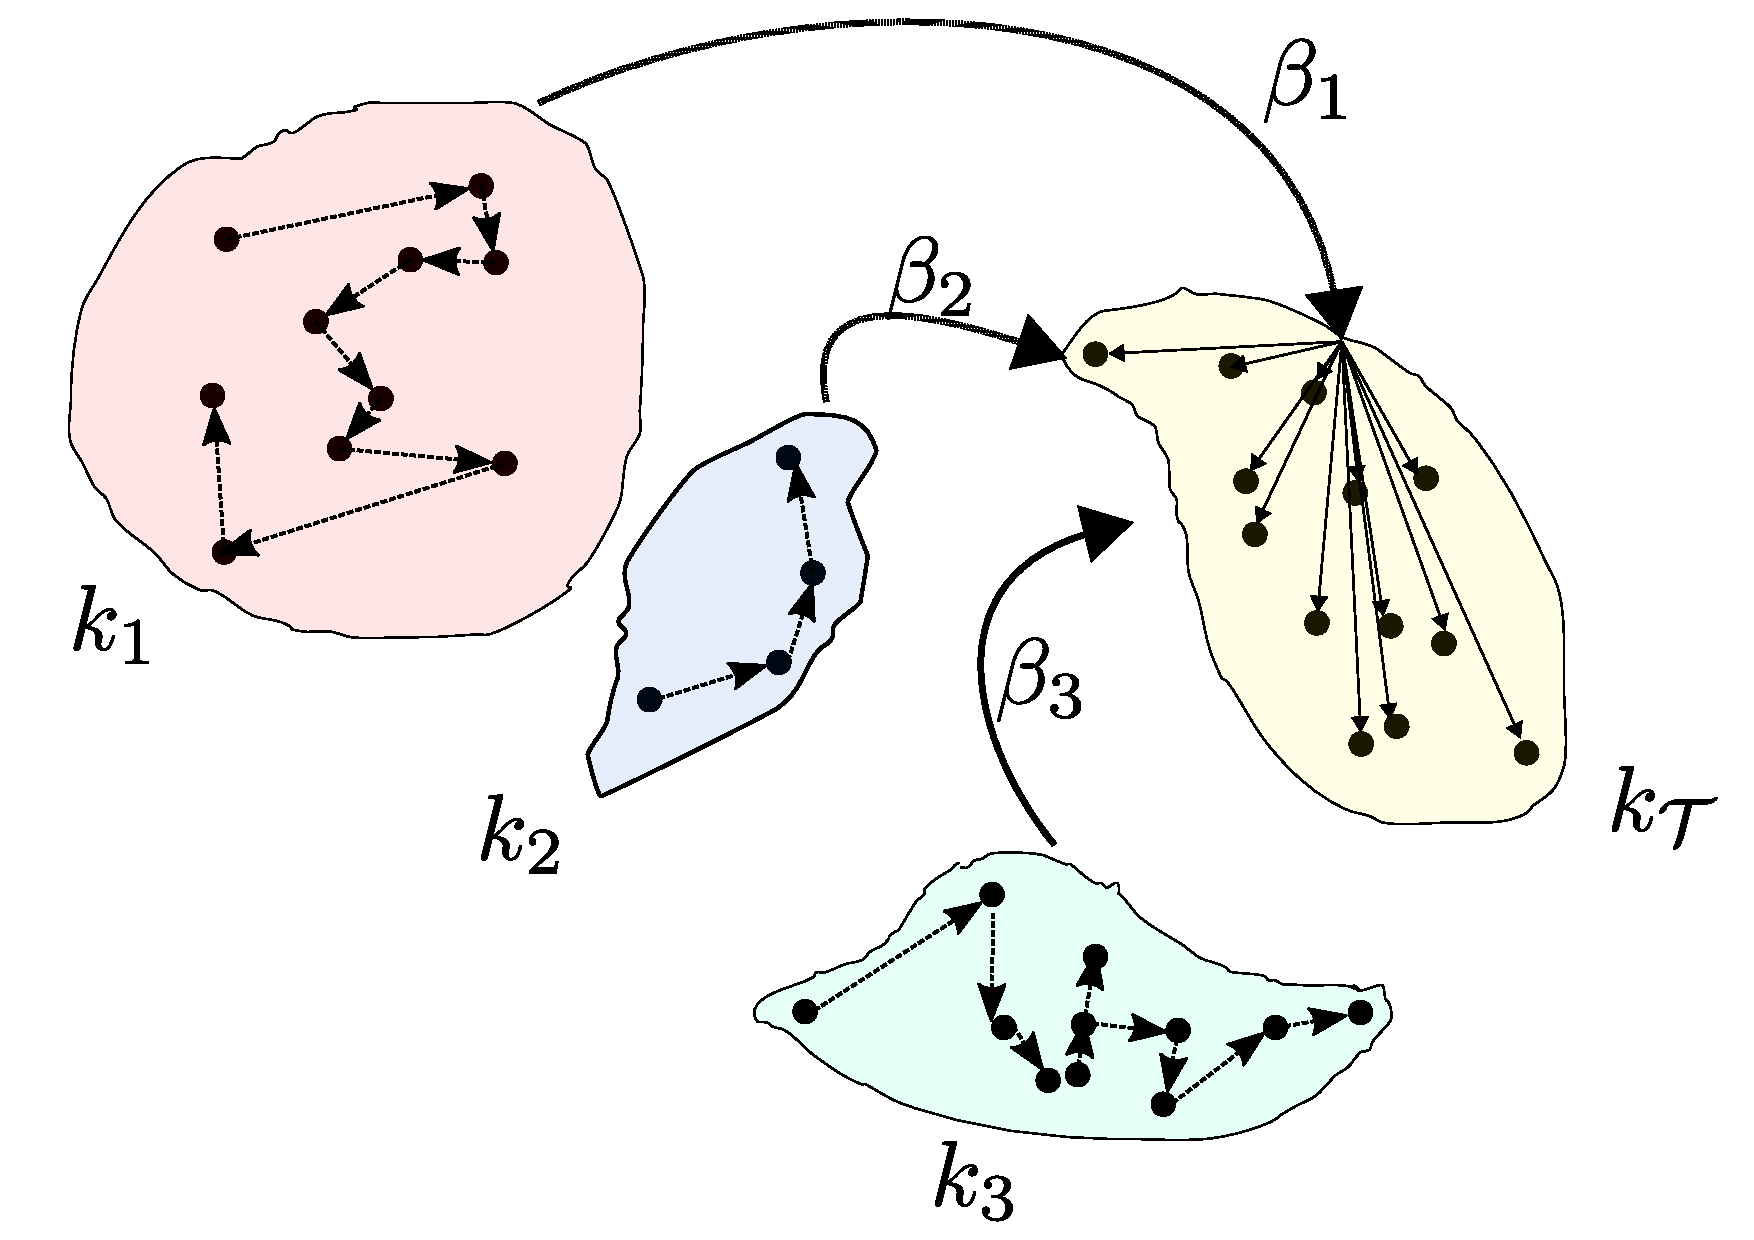
\includegraphics[width= 0.80\columnwidth]{fig/cluster_knowledge_transfer.pdf} \label{fig:cluster_knowledge_transfer}}
	\hspace*{\fill}
	\caption[] {\label{fig:tranfer_learninhg} Transfer learning. \subref{fig:effect_transfer_learning} The effect of transfer learning, \subref{fig:cluster_knowledge_transfer} transfer of knowledge from different origin clusters to the target cluster.}
\end{figure*}
% ---
% ---------------------------------------------------------------------------------------------------
\subsubsection{\textbf{Incremental learning (I)}}
Following Assumption~\ref{assumption:skill_clustering}, skills with comparable similarity are clustered in $\mathcal{K} = \lbrace k_i \rbrace^{N_\mathcal{K}}_{i=1} $ clusters, with $N_\mathcal{K}$ being the total number of clusters, see Fig.~\ref{fig:incremental_transfer_similarity}. Any two skills belonging to different clusters cannot profit from incremental learning algorithms in virtue of their relatively low similarity. Thus, with \eqref{eq:incremental_knowledge}, the scaling effect that incremental learning has on the skill complexity $c_j$ for the skills contained in the $i$-th cluster is
% ---
%\begin{equation}\label{eq:complexity_IL}
%  {^k}c^{(I)}_j = c_0 \cdot {^k}\bar{\sigma}_j = c_0 \left( e^{-\alpha \cdot {^kN_{j}}}\right)^r = c_0 \left( e^{-\alpha \cdot {^kN_{j}}}\right),
%\end{equation}
\begin{equation}\label{eq:complexity_IL}
	c^{(I)}_{j,k} = c_0 \cdot \bar{\sigma}_{j,k} = c_0 \left( e^{-\alpha \cdot {N_{j,k}}}\right)^r = c_0 \left( e^{-\alpha \cdot {N_{j,k}}}\right),
\end{equation}
% ---
\textcolor{red}{where $r=1$} and ${N_{j,k}}$ indicates the number of already learned skills in the $k$-th cluster. The effect on complexity is shown in Fig.~\ref{fig:complexity_per_cardinality}. Similarly, $\bar{\sigma}_{j,k}$ indicates the knowledge that is yet to be acquired about a given skill in cluster $k$. \textcolor{red}{In virtue of the high similarity of the skills in the cluster, the term $\left(1-\bar{\sigma}_{j,k}\right)$ indirectly reflects the knowledge collected from the skills in the $k$-th cluster.}

The total number of trial episodes $ C_k $ that an agent following an incremental learning strategy needs to learn the skills in a cluster $ k $ is given by
% ---
%\begin{align}
%	\begin{split}
%		C^{(I)}_k &= \sum^{N_\mathcal{S}/N_\mathcal{K}}_{j=1} c_0 \cdot e^{-\alpha \cdot {^kN_{j}}} = \sum^{N_\mathcal{S}/N_\mathcal{K}}_{j=1}c_0 \cdot e^{-\alpha {^{k}\cancelto{j-1}{N_{j}}}}\\
%		&= c_0 \sum^{N_\mathcal{S}/N_\mathcal{K}}_{j=1} e^{-\alpha (j-1)}.
%	\end{split}
%\end{align}
\begin{align}
	\begin{split}
		C^{(I)}_k &= \sum^{N_\mathcal{S}/N_\mathcal{K}}_{j=1} c^{(I)}_{j,k}  \\
		&= \sum^{N_\mathcal{S}/N_\mathcal{K}}_{j=1} c_0 \cdot  \bar{\sigma}_{j,k}  = \sum^{N_\mathcal{S}/N_\mathcal{K}}_{j=1} c_0 e^{-\alpha {\cancelto{j-1}{N_{j,k}}}}\\
		&= c_0 \sum^{N_\mathcal{S}/N_\mathcal{K}}_{j=1} e^{-\alpha (j-1)}.
	\end{split}
\end{align}
% ---
Likewise, the total number of episodes to learn the skills in all the $ N_\mathcal{K} $ clusters is
%\begin{align}\label{eq:complexity_incremental_single}
%	\begin{split}
%	C^{(I)} &= N_\mathcal{K} \cdot c_0 \frac{1 - e^{-\alpha \frac{N_\mathcal{S}}{N_\mathcal{K}}}}{1 - e^{-\alpha}}\\
%&= N_\mathcal{K} \cdot c_0 \frac{1 - \bar{\sigma}^{(I)}}{1 - e^{-\alpha}}.
%	\end{split}
%
%\end{align}
\begin{align}\label{eq:complexity_incremental_single}
	\begin{split}
		C_\mathcal{S}^{(I)} &= N_\mathcal{K} \cdot c_0 \frac{1 - e^{-\alpha \frac{N_\mathcal{S}}{N_\mathcal{K}}}}{1 - e^{-\alpha}}\\ 
		&= N_\mathcal{K} \cdot c_0 \frac{1 - \bar{\sigma}_k^{(I)}}{1 - e^{-\alpha}}.
	\end{split}
\end{align}
% ---
with $ \bar{\sigma}^{(I)}_k = e^{-\alpha \frac{N_\mathcal{S}}{N_\mathcal{K}}} $ representing the knowledge remaining after learning all the skills in a cluster. If $ m $ robots are available, each agent can take care of learning $ \frac{N_\mathcal{S}}{m \cdot N_\mathcal{K}} $ skills in parallel with the rest. Under such conditions, the total number of episodes is simply
% ---
\begin{align}\label{eq:complexity_incremental_parallel}
	\begin{split}
		{}^{\lvert \lvert}C_\mathcal{S}^{(I)} &= m \cdot N_\mathcal{K} \cdot c_0 \frac{1 - e^{-\alpha \frac{N_\mathcal{S}}{m \cdot N_\mathcal{K}}}}{1 - e^{-\alpha}} \\
		&= m \cdot N_\mathcal{K} \cdot c_0 \frac{1 - \bar{\sigma}^{(I)}_m}{1 - e^{-\alpha}} 	
	\end{split}	
\end{align}
%---
\begin{table*}[htbp!]
	\begin{center}
		\captionof{table}{The complexity of the different learning schemes.} \label{tab:method_comparison}
		\begin{tabular}{|c|c|c|c| } 
			\multicolumn{4}{c}{$\left[1- \sum\limits_{k \in \mathcal{K} \setminus k_\mathcal{T}}\beta_k \left( 1 - \bar{\sigma}_{j,k} \right)\right] \left(e^{-\alpha N_{j,k_\mathcal{T}}} \right)^r$}\\
			\multicolumn{3}{c}{}\\
			\hline
			\cellcolor{black!25} & \textbf{Incremental} & \textbf{Transfer} & \textbf{Collective}\\
			
			\cellcolor{black!25} & $r=1, \quad \beta_k=0$ & $r=1$ & $r=m, \quad \mathcal{K} \setminus k_\mathcal{T}=\emptyset, \quad N_{j,k_\mathcal{K}} = N_j$\\
			\hline 
			Single & $ C_\mathcal{S}^{(I)} = N_\mathcal{K} \cdot c_0 \frac{1 - e^{-\alpha \frac{N_\mathcal{S}}{N_\mathcal{K}}}}{1 - e^{-\alpha}}  $ 
			& $C_\mathcal{S}^{(T)}= \left[1 - \frac{\left(1+N_\mathcal{K}\right)}{2}\beta \left(1-\bar{\sigma}\right)\right] C_\mathcal{S}^{(I)}$& \multirow{2}{*}{${^{\vert \lvert}}C_\mathcal{S}^{(C)} = m \cdot c_0 \frac{1 - e^{-\alpha N_\mathcal{S}}}{1 - e^{-\alpha m}}$}\\
			%\hline
			Parallel & $ {^{\vert \lvert}}C_\mathcal{S}^{(I)} = m \cdot N_\mathcal{K} \cdot c_0 \frac{1 - e^{-\alpha \frac{N_\mathcal{S}}{m \cdot N_\mathcal{K}}}}{1 - e^{-\alpha}}  $ 
			& ${^{\vert \lvert}}C_\mathcal{S}^{(T)} = \left[1 - \frac{\left(1+N_\mathcal{K}\right)}{2}\beta \left(1-\bar{\sigma}_m\right)\right] {^{\vert \lvert}}C_\mathcal{S}^{(I)}$ & \\
			\hline
		\end{tabular}
	\end{center}
	%\label{tab:method_comparison}
\end{table*}
% ---------------------------------------------------------------------------------------------------
\subsubsection{\textbf{Transfer learning (TL)}}

%\begin{figure}[!h]
%	\centering
%	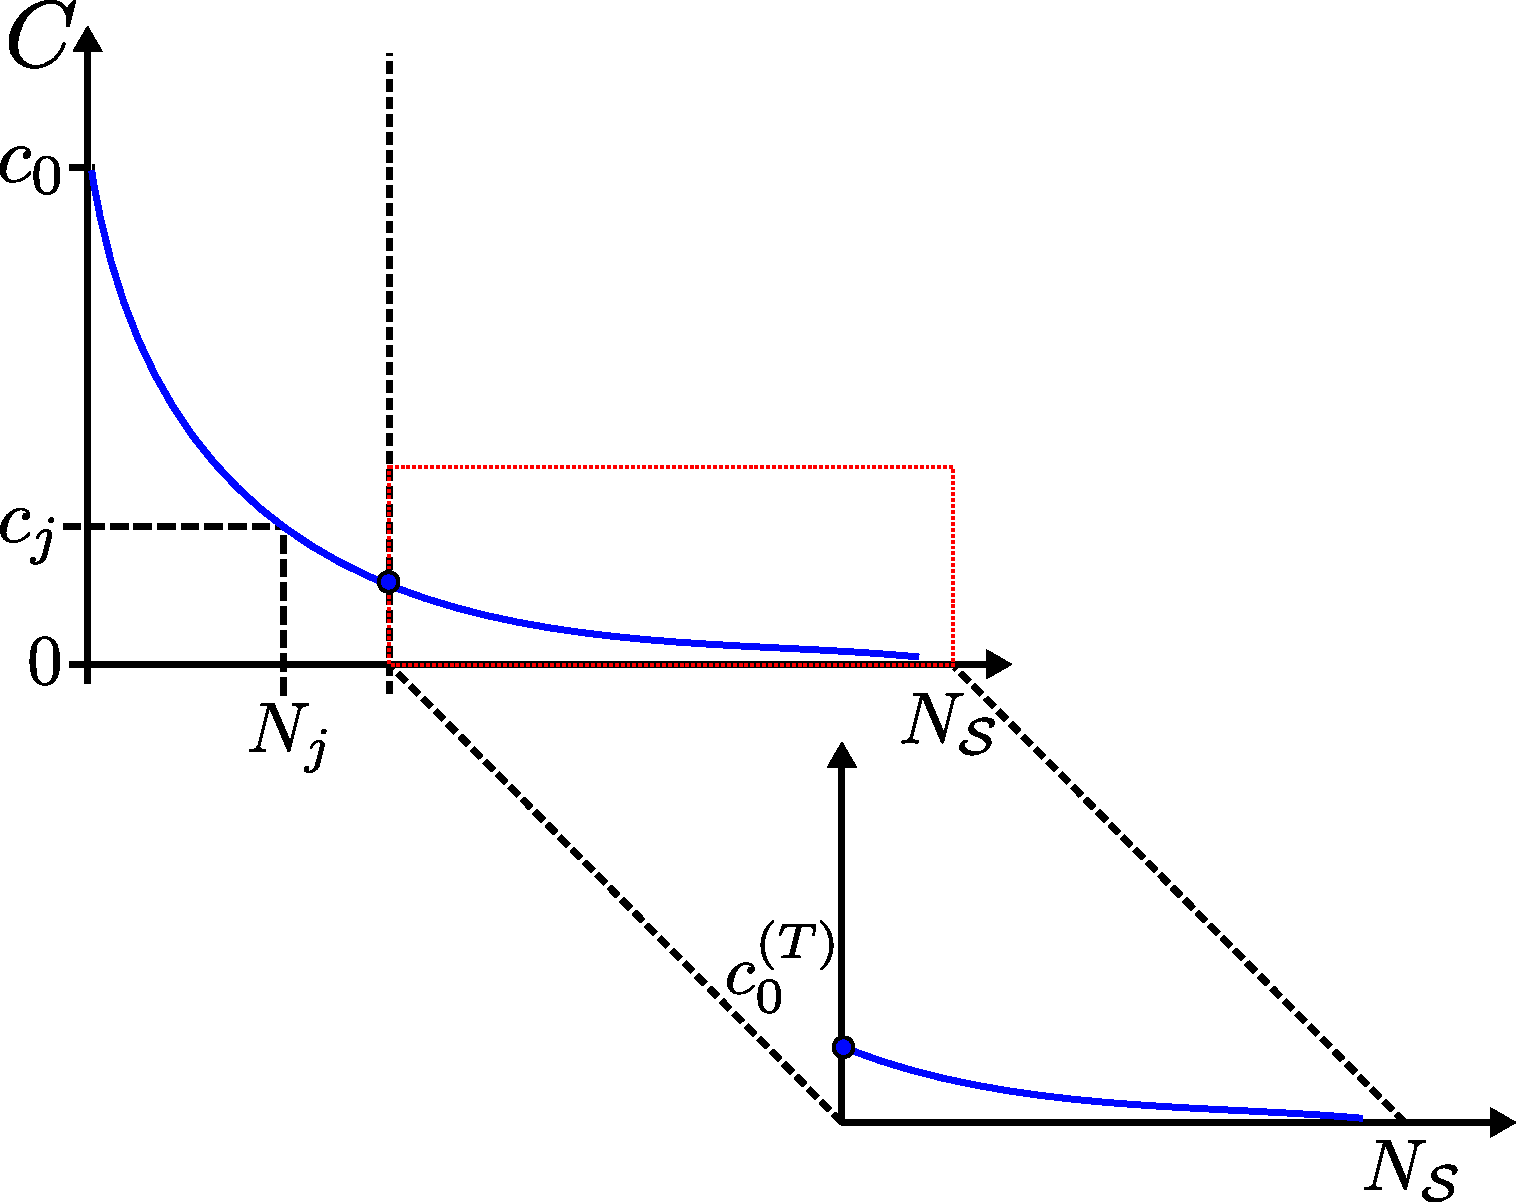
\includegraphics[width=0.9\columnwidth]{fig/effect_transfer_learning.pdf}
%	\caption{The effect of transfer learning.}
%	\label{fig:effect_transfer_learning}
%\end{figure}
%---
TL represents the exchange of knowledge from the skills learned in different \emph{origin} clusters $\mathcal{O}$ to the skills that will be learned in a \emph{target} cluster $\mathcal{T}$, see Fig.~\ref{fig:incremental_transfer_similarity}. In general, the effect that TL has on the skills of another cluster is the reduction of the total remaining knowledge to be learned. Referring to \eqref{eq:incremental_knowledge}, it means that its value when $N_{j,k} = 0$ will be reduced (Fig.~\ref{fig:effect_transfer_learning}). Considering $\mathcal{K} = \{ k_i \}^{N_\mathcal{K}}_{i=1}$ to be the set of all available clusters of knowledge (see Fig.~\ref{fig:cluster_knowledge_transfer}), the TL effect can be modeled as follows
% ---
\begin{align}
	\begin{split}
		\bar{\sigma}^{(T)}_{j,k_\mathcal{T}} &= \left\{ e^{-\alpha \left(N_{j,k_\mathcal{T}} - \frac{1}{\alpha \cdot r}  \log\left[ 1- \sum\limits_{k\in \mathcal{K} \setminus k_\mathcal{T}}\beta_k(1 - \bar{\sigma}_{j,k}) \right] \right)}\right\}^r\\
		&= \left(e^{-\alpha {N_{j,k_\mathcal{T}}}} \right)^r e^{  \log\left( 1-\sum\limits_{k \in \mathcal{K} \setminus k_\mathcal{T}}\beta_k(1 - \bar{\sigma}_{j,k}) \right) }\\
		&= \underbrace{\left[1- \sum\limits_{k \in \mathcal{K} \setminus k_\mathcal{T}}\beta_k \left( 1 - \bar{\sigma}_{j,k} \right)\right]}_{\text{Transfer}} \left(e^{-\alpha N_{j,k_\mathcal{T}}} \right)^r ,
	\end{split}
\end{align}
% ---
where $0<\beta_k << 1$ is the transfer coefficient from the different $\mathcal{O}$ clusters to the $\mathcal{T}$ cluster. Additionally,
% ---
\begin{equation}
    \sum\limits_{k \in \mathcal{K} \setminus k_\mathcal{T}}\beta_k \leq 1,
\end{equation}
% ---
assuming that the origin clusters have unique knowledge contributions to the target cluster. \textcolor{red}{Again, $ r = 1 $ in this case.} Furthermore, considering Assumptions~\ref{assumption:cluster_size} and \ref{assumption:cluster_transferability} $ \beta_k = 1/\rvert \mathcal{K} \setminus k_\mathcal{T} \lvert$ and $ \bar{\sigma}_{j,k} = \bar{\sigma}_m $. Where $ \bar{\sigma}_m $ represents the knowledge collected from the other clusters; i.e.
% ---
\begin{equation}
	\bar{\sigma}_m = e^{-\alpha \frac{N_\mathcal{S}}{m N_\mathcal{K}}}.
\end{equation}

Similar to incremental learning, the total number of trial episodes required to learn all the skills in the $ N_\mathcal{K} $ clusters is
% ---
\begin{align}\label{eq:complexity_transfer_single}
	C_\mathcal{S}^{(T)} &= \left[1 - \frac{\left(1+N_\mathcal{K}\right)}{2}\beta \left(1-\bar{\sigma}^{(I)}_k\right)\right] N_\mathcal{K} \cdot  c_0 \frac{1 - e^{-\alpha \frac{N_\mathcal{S}}{N_\mathcal{K}}}}{1 - e^{-\alpha}}\\
	&= \left[1 - \frac{\left(1+N_\mathcal{K}\right)}{2}\beta \left(1-\bar{\sigma}^{(I)}_k\right)\right] N_\mathcal{K} \cdot  c_0 \frac{1 - \bar{\sigma}^{(I)}_k}{1 - e^{-\alpha}}	
\end{align}
% ---
Furthermore, if $ m $ robots can be used in parallel to learn th skills in the clusters; then
% ---
\begin{equation}\label{eq:complexity_transfer_parallel}
	{}^{\lvert \lvert}C_\mathcal{S}^{(T)} = \left[1 - \frac{\left(1+N_\mathcal{K}\right)}{2}\beta \left(1-\bar{\sigma}_m\right)\right] m \cdot N_\mathcal{K}  \cdot c_0 \frac{1 - e^{-\alpha \frac{N_\mathcal{S}}{m \cdot N_\mathcal{K}}}}{1 - e^{-\alpha}},
\end{equation}
% ---
% ---------------------------------------------------------------------------------------------------
\subsubsection{\textbf{Collective learning (TL)}}
Finally, in collective learning the notion of cluster is not necessarily applicable anymore, thus 
$\mathcal{K} = k_\mathcal{T}$ which corresponds to the existence of only one big cluster.
% ---
\begin{align}
	\begin{split}
		\bar{\sigma}^{(C)} &=   \cancelto{1}{ \left[1- \sum_{k \in \mathcal{K} \setminus k_\mathcal{T}}\beta_k \left( 1 - \bar{\sigma}_{j,k} \right)\right]} \left(e^{-\alpha {{^\mathcal{T}}N_j}} \right)^r \\%e^{-\alpha ^\mathcal{T}N_j}\\
		&= \left(e^{-\alpha N_{j,k_\mathcal{T}}} \right)^r  = \left(e^{-\alpha N_{j}}\right)^r 
	\end{split}
\end{align}

Furthermore, now $m$ robots are learning (potentially) $m$ different skills in parallel while exchanging knowledge.
% ---
\begin{align}
\begin{split}
    \bar{\sigma}^{(C)} &= \left({e^{-\alpha \cdot N_j}}\right)^{r}\\
    &= \left({e^{-\alpha \cdot N_j}}\right)^{m}.
\end{split}
\end{align}
% ---
%where $\alpha$ was replaced by $ 0<\gamma<<1$, which models a more effective knowledge transfer among the $m$ agents.}

The total number episodes when using collective learning is given by
% ---
\begin{eqnarray}
	C_\mathcal{S}^{(C)} = m \cdot C_0 \frac{1 - e^{-\alpha N_\mathcal{S}}}{1 - e^{-\alpha m}}
\end{eqnarray}
% ---
% ===================================================================================================
\subsection{Comparison}
 The general complexity scaling based on knowledge sharing expression is
\begin{tcolorbox}
	\begin{align}
		c_j &= c_0\left[1- \sum\limits_{k \in \mathcal{K} \setminus k_\mathcal{T}}\beta_k \left( 1 - \bar{\sigma}_{j,k} \right)\right] \left(e^{-\alpha N_{j,k_\mathcal{T}}} \right)^r
	\end{align}
\end{tcolorbox}
 where according to \eqref{eq:learning_combinations}, the effects of the different learning schemes are reflected.
 % ---
 \begin{equation}
	 c_j =
	     \begin{cases} 
		       \text{Incremental} & \alpha\neq 0, \beta=0,  r=1 \\
		       \text{Transfer} & \alpha\neq 0, \beta \neq 0, r = 1 \\
		       \text{Collective} & \alpha\neq 0, \beta = 0, r=m 
		   \end{cases}
	   \label{eq:learning_combinations}
\end{equation}
From \eqref{eq:complexity_incremental_parallel} and \eqref{eq:complexity_transfer_parallel} it is clear that they differ only by the factor $ \left[1 - \frac{\left(1+N_\mathcal{K}\right)}{2}\beta \left(1-\bar{\sigma}_m\right)\right] \leq 1$, showing that TL is a scaled down version of IL. Table~\ref{tab:method_comparison} shows the comparison between the total number of trial episodes required by the three learning schemes.

% ---
The total energy and time consumption in the different learning paradigms is
% ---
\begin{align}
	\begin{split}
		E^{(\star)}_{\mathcal{S}} &= e_{0} \cdot {}^{\lvert \lvert}C_\mathcal{S}^{(\star)}\\
		T^{(\star)}_{\mathcal{S}} &= \frac{\Delta t}{m} \cdot {}^{\lvert \lvert}C_\mathcal{S}^{(\star)},
	\end{split}
\end{align}
% -----
with $ \star $ representing the total complexity corresponding the considered learning scheme.

%\begin{algorithm}
%\caption{Learning algorithm}\label{alg:cap}
%\begin{algorithmic}
%\Require $n \geq 0$
%\Ensure $y = x^n$
%\State $y \gets 1$
%\State $X \gets x$
%\State $N \gets n$
%\While{$\lvert \bar{\mathcal{K}} \lvert  < \lvert {\mathcal{K}}\lvert$}
%\State Choose a cluster $k_\mathcal{T} \notin \bar{\mathcal{K}}$
%\If{$\bar{\mathcal{K}} \neq \emptyset$}
%    %\State $\kappa \gets \text{aggregate_knowledge}(\bar{\mathcal{K}})$ \Comment{Integrate knowledge from origin clusters}
%    \State ${^\mathcal{T}\bar{\sigma}(0)} \gets \text{transfer_knowledge}(\kappa)$ \Comment{Define new initial point}
%\EndIf
%\For{\texttt{<some condition>}}
%\State \texttt{<do stuff>}
%\EndFor    
%\EndWhile
%\end{algorithmic}
%\end{algorithm}



%$\prescript{14}{2}{\mathbf{C}} $ For large operators, use from amsmath $ \sideset{_a^b}{'}\sum A_n $


% ===================================================================================================
% \subsection{General expression}
% The general complexity scaling based on knowledge sharing expression is
% \begin{tcolorbox}
% \begin{align}
%          c_j &= c_0\bar{\sigma}^{(C)}\\
%          &= c_0\left[1-\beta_k \left( 1 - \bar{\sigma}_O \right)\right]e^{-\alpha N_j},
% \end{align}
% \end{tcolorbox}
% where according to \eqref{eq:learning_combinations}, the effects of the different learning schemes are reflected.
% % ---
% \begin{equation}
% c_j =
%     \begin{cases} 
%       \text{Isolated} & \alpha=\beta=m =0 \\
%       \text{Incremantal} & \alpha\neq 0, \beta=m =0 \\
%       \text{Incremental + Transfer} & \alpha\neq 0, \beta \neq 0, m = 0 \\
%       \text{Collective} & \alpha\neq 0, \beta = 0, m \neq 0 
%   \end{cases}
%   \label{eq:learning_combinations}
% \end{equation}

%\Xhline{5\arrayrulewidth}

% % \pagebreak
% \begin{tcolorbox}
% 	\begin{assumption}\label{assumption:incremental_similarity} Under incremental learning, the level of observable similarity among the considered skills in a cluster is comparable.
% 	\end{assumption}
% \end{tcolorbox}
% % --- 
% \begin{tcolorbox}
% 	\begin{assumption}\label{assumption:exponential_effect} The knowledge function $\bar{\sigma}(\cdot)$, describing the knowledge that remains to be learned about a skill, has an exponentially decreasing behavior.
% 	\end{assumption}
% \end{tcolorbox} 
% % ---
% Considering Assumptions \ref{assumption:incremental_similarity} and \ref{assumption:exponential_effect}, an idealization of the behavior described by \eqref{eq:knowledge_limit} can be modeled as a decreasing exponential which is a function of the number of already learned skills from the cluster $k$; i.e. ${^kN_j}$:
% % ---
% % \begin{equation}\label{eq:incremental_knowledge}
% %   {^k}\bar{\sigma}^{(I)}_j = e^{-\alpha  \cdot {^k}N_{j}} \in (0,1],
% % \end{equation}
% % ---
% \begin{align}
%     \bar{\sigma}^{(C)} &= e^{-\alpha  \left(m \cdot N_j - \frac{1}{\alpha}  \log\left( 1- \beta_k(1 - \bar{\sigma}_O) \right) \right)}\\
%          &= e^{-\alpha  \cdot m \cdot N_j}e^{  \log\left( 1-\beta_k(1 - \bar{\sigma}_O) \right) }\\
%          &= \left[1-\beta_k \left( 1 - \bar{\sigma}_O \right)\right]e^{-\alpha \cdot m\cdot N_j}
% \end{align}
% % ---
% %\textcolor{red}{Plugging \eqref{eq:similarity_metric} into \eqref{eq:scaled_complexity}, it is easily seen that the complexity decreases exponentially, see Fig.~\ref{fig:complexity_per_cardinality}}.
% \hl{where $ 0<\alpha<<1$ models how effectively the knowledge contained in $\mathcal{S}_j$ is shared with $s_j$.} 
% % ---
% \begin{equation}\label{eq:complexity_TL}
%   {^k}c^{(I)}_j = c_0 \cdot {^k}\bar{\sigma}^{(I)}_j = c_0 \cdot e^{-\alpha \cdot ^kN_{j}}
% \end{equation}
% % ---
% % If a batch of $m$ robots executes incremental learning; then, $ {^kN_{j}} = ({^k}j-1)$. Where $^kN_{j}}$ is the number of already leaned skill within a cluster. Therefore, the total energy for the batch of robots learning all the skills in the batch is then,
% If a batch of $m$ robots executes incremental learning, each robot in the batch will learn $^kN_\mathcal{S}$; where ${^kN_\mathcal{S}}$ is the number of skills in the cluster. Therefore, the total energy for the batch of robots learning all the skills in the batch is then,
% % ---
% \begin{equation}
%   {^k}E^{(I)}_j = {^km} \cdot c_0 \cdot e_0 \cdot \left.{^k}\bar{\sigma}^{(I)}_j \right\vert_{{^k}N_j = j-1}.
% \end{equation}
% % ---
% where ${^km}$ is the number of robots assigned to learn the skills in a cluster.  

% \important{To simplify the expressions we are assuming that ${^kN_\mathcal{S}}$ is divisible by ${^km}$.}

% By extension, the total energy expenditure is
% % ---
% \begin{align}\label{eq:itl_total_energy}
% \begin{split}
%   E^{(I)}_{\mathcal{S}} &= \sum^{K_\mathcal{O}}_{k=1}  \left( {\sum^{{{^k}N_{\mathcal{S}}}/{{^k}m}}_{j=1} {^k}E^{(I)}_j} \right)
%   \\
%   %& = m \cdot e_o  \cdot c_0 \sum^{{N_{\mathcal{T}}}/{m}}_{j=1} e^{- \alpha m (j-1) } \\
%   %& = m \cdot e_0 \cdot c_0 \cdot \left(\frac{1 - e^{ - \alpha N_{\mathcal{T}}}}{1 - e^{-\alpha m}}\right) 
% \end{split}
% \end{align}
% % ---

% % ===================================================================================================
% \subsubsection{Transfer learning}
% Transfer learning is the class of learning algorithms that can leverage skill similarity in the latent space. Just like in the observable space, latent similarity is used to define the clusters of skills $\lbrace k \rbrace^{K_\mathcal{L}}_1 $ in the latent space, with $1 \leq K_\mathcal{L} \leq K_\mathcal{O}$. The set of expression to compute the energy demand to learn all the $N_\mathcal{S}$ skills is analogous to that of incremental learning; i.e.:
% % ---
% \begin{align}
%     \bar{\sigma}^{(I+T)} &= e^{-\alpha \left(N_j - \frac{1}{\alpha}  \log\left( 1- \beta_k(1 - \bar{\sigma}_O) \right) \right)}\\
%          &= e^{-\alpha N_j}e^{  \log\left( 1-\beta_k(1 - \bar{\sigma}_O) \right) }\\
%          &= \left[1-\beta_k \left( 1 - \bar{\sigma}_O \right)\right]e^{-\alpha N_j}
% \end{align}


% \begin{align}
%     \bar{\sigma}^{(C)} &= e^{-\alpha  \left(m \cdot N_j - \frac{1}{\alpha}  \log\left( 1- \beta_k(1 - \bar{\sigma}_O) \right) \right)}\\
%          &= e^{-\alpha  \cdot m \cdot N_j}e^{  \log\left( 1-\beta_k(1 - \bar{\sigma}_O) \right) }\\
%          &= \left[1-\beta_k \left( 1 - \bar{\sigma}_O \right)\right]e^{-\alpha \cdot m\cdot N_j}
% \end{align}




% \begin{equation}
%     \bar{\sigma}^{(I+T)} = e^{-\alpha N_j}\cdot \overbrace{\left( (1- \beta_k) \cdot \underbrace{e^{-\alpha_k N^k_j}}_{\bar{\sigma}_k}\right) }^{\text{Transfer}}
% \end{equation}

% % ---
% \begin{align}
%     \bar{\sigma}^{(I+T)} &= \underbrace{e^{-\alpha N_j}}_{\bar{\sigma}_T}\cdot \overbrace{\left( 1- \beta_k \cdot \underbrace{e^{-\alpha_k N^k_j}}_{\bar{\sigma}_O}\right) }^{\text{Transfer}}\\
%     &= \bar{\sigma}_T - \beta \bar{\sigma}_T \bar{\sigma}_O\\
%     &= (1 - \beta \cdot \bar{\sigma}_O) \bar{\sigma}_T
% \end{align}



% % ---
% \begin{subequations}\label{eq:cl_total_energy}
% \begin{align}
% {^k}\bar{\sigma}^{(T)}_j &= e^{-\alpha  \cdot {^k}N_{j}} \in (0,1],\\
% {^k}c^{(T)}_j &= c_0 \cdot {^k}\bar{\sigma}^{(T)}_j = c_0 \cdot e^{-\alpha \cdot ^kN_{j}}\\\label{eq:complexity_TL}
%   {^k}E^{(T)}_j &= {^km} \cdot c_0 \cdot e_0 \cdot \left.{^k}\bar{\sigma}^{(T)}_j \right\vert_{{^k}N_j = j-1}\\
%   E^{(T)}_{\mathcal{S}} &= \sum^{K_\mathcal{L}}_{k=1}  \left( {\sum^{{{^k}N_{\mathcal{S}}}/{{^k}m}}_{j=1} {^k}E^{(T)}_j} \right)
% \end{align}
% \end{subequations}

% % ===================================================================================================
% \subsubsection{Collective learning}
% Now, let $\mathcal{S}_\mathcal{L} = \lbrace \hat{s}_i\rbrace^n_{i=1}$ define the set containing all the latent (or basis) skills that can be composed to accomplish any skill, where each latent skill is independent of the other; i.e. they are the dimensions of the latent space $\mathcal{L}$. \hl{Furthermore, every task $s_i \in \mathcal{S}$ is composed of of a subset $\mathcal{A}_j$ of primitive skills from $\mathcal{S}_\mathcal{L}$; i.e. $ \mathcal{A}_j \subset \mathcal{S}_\mathcal{L} $. }
% % ---
% \begin{tcolorbox}
% 	\begin{definition}\label{definition:complexity} A skill $s_i$ can be defined by \textcolor{red}{composing/aggregating} a set of latent skills $\mathcal{A}_j$.
% 	\end{definition}
% \end{tcolorbox}
% % ---
% To simplify the analysis, we assume that each skill is composed of a fixed number $m$ of latent skills; i.e $|\mathcal{A}| = m$. The knowledge about each latent skill $s_i$ is defined $ \kappa_i \in (0,1) $.

% \subsubsection{Skill knowledge}

% Consider a function ${\phi}_i(\hat{s}_i)\in [0,1)$ that expresses the knowledge from a latent skill  $\hat{s}_i \in \mathcal{S}_\mathcal{L}$. \textcolor{red}{We assume that the knowledge about $\hat{s}_i$ is \hl{exponentially} proportional to the number of times $ l_i $ which this latent skill was required by the skills in the set of previously learned skills $\mathcal{S}_j \subset \mathcal{S}$}.
% % that \hl{\textbf{is not}} contained in a set of already learned tasks $\mathcal{T}_j \subset \mathcal{T}_j \subset \mathcal{T}$. 
% The function ${\phi}_i(\cdot)$ satisfies:
% \begin{itemize}
% 	\item ${\phi}_i(\hat{s}_i) = 0$, if $\mathcal{S}_j=\emptyset$ or if it does not contain knowledge about the latent skill $\hat{s}_i$
% 	\item ${\phi}_i(\hat{s}_i) = 1$, if all the knowledge about $\hat{s}_i$ is contained in $\mathcal{S}_j$
% \end{itemize} 
% %Conceptually, ${\sigma}_j(\mathcal{T}_j)$ \textcolor{red}{is the fraction of knowledge that remains to be learned.}
% The knowledge function is defined as follows
% \begin{equation}\label{eq:knowledge_function}
% \phi_i(\hat{s}_i) = 1 - e^{-\beta_i l_i},
% \end{equation}
% where $ l_i $ is computed as
% % ---
% \begin{equation}\label{eq:repetition_summation}
% l_i = \sum_{k = 1}^{j} f(\hat{s}_i,\mathcal{A}_k)
% \end{equation}
% with $ f(\hat{s}_i,\mathcal{A}_k) $ being
% % ---
% \begin{equation}\label{eq:repetition}
% f(\hat{s}_i,\mathcal{A}_k) =
% \begin{cases} 
% 1 & \hat{s}_i \in \mathcal{A}_k\\
% 0 & \hat{s}_i \notin \mathcal{A}_k
% \end{cases}
% \end{equation}
% % ---
% The knowledge about a latent skill is analogous to the probability of successfully executing the latent skill; i.e. 
% \important{Replace symbol with \emph{is equivalent to}}
% \begin{equation*}
% \phi_j \equiv p(\hat{s}_j)
% \end{equation*}

% \subsubsection{Skill knowledge}

% \important{Monotonic}
% Given the independence assumption on the skills $ \hat{s}_i $, the knowledge $ \kappa_j \in [0,1]$ about a skill $ s_j $ is the product of the knowledge $ \phi_k $ from its composing latent skills; i.e.
% % \begin{equation}
% % \kappa_j = \prod_k \phi_k(\hat{s}_k) \quad \forall \hat{s}_k \in \mathcal{A}_j  
% % \end{equation}
% \begin{equation}
% \bar{\sigma}^{(C)}_j =1 - \underbrace{\prod_k \phi_k(\hat{s}_k) }_{\text{acquired knowledge}}   \quad \forall \hat{s}_k \in \mathcal{A}_j
% \end{equation}


% \newpage
% \pagebreak
% \hline


% % ===================================================================================================
% \subsection{Energy and time demand for learning tasks}
% % % ---
% % \begin{figure}[!ht]
% % 	\centering
% % 	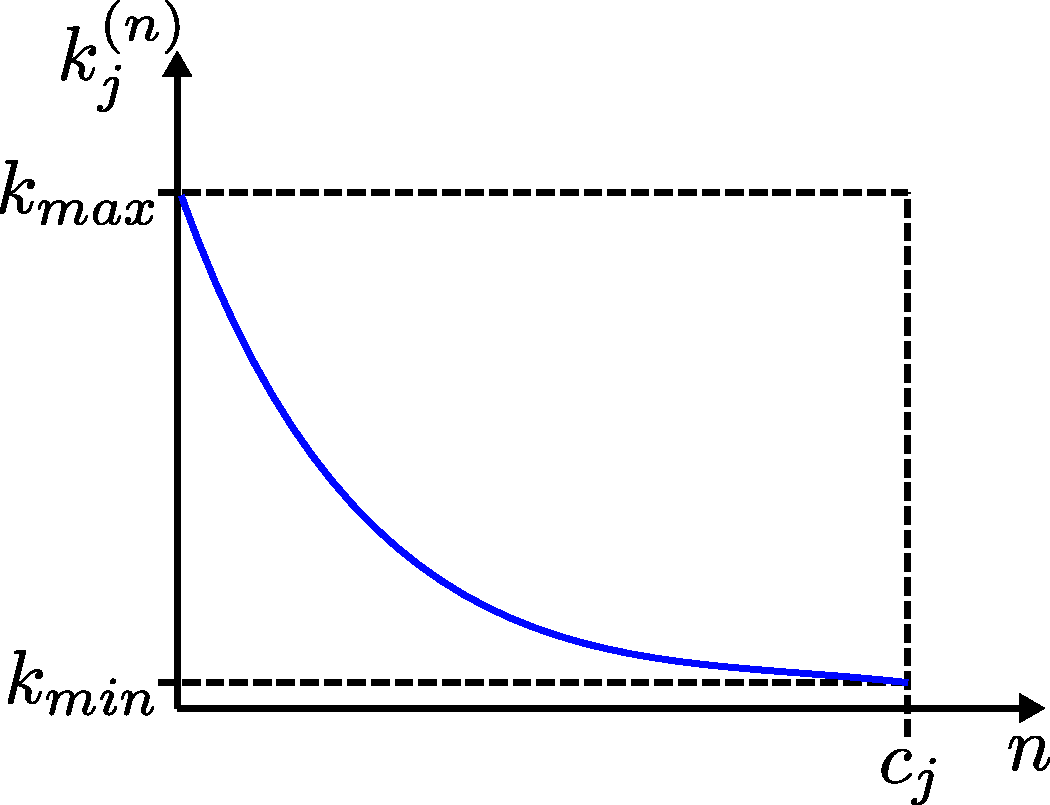
\includegraphics[width=0.7\columnwidth]{fig/steps_per_episode.pdf}
% % 	\caption{The number of time steps required to solve a task decreases with the number of episodes. $c_j$ is the max. number of episodes that it takes to learn a task.}
% % 	\label{fig:timesteps_per_episode}
% % \end{figure}
% % % ---

% % ---
% \begin{figure}[!ht]
% 	\centering
% 	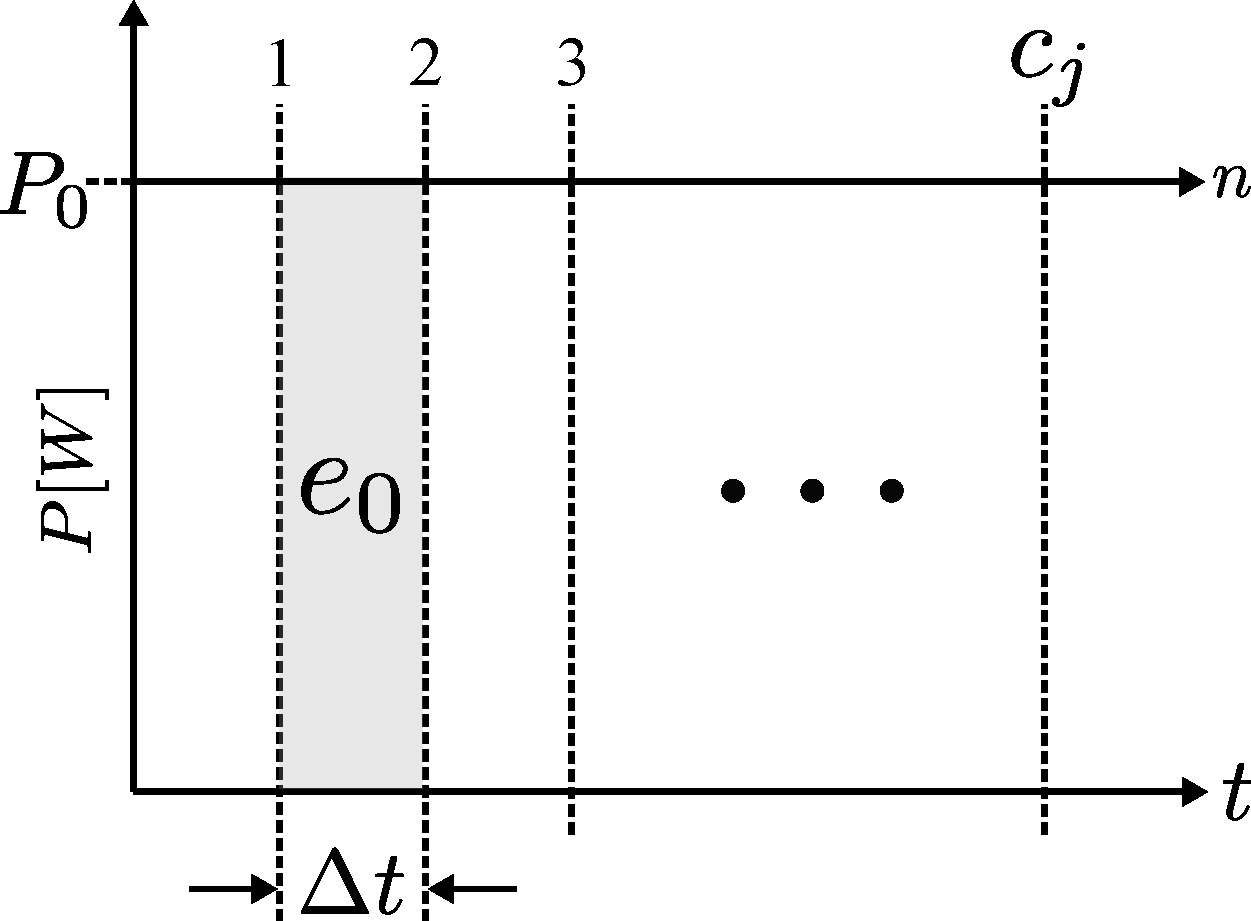
\includegraphics[width=0.9\columnwidth]{fig/power_per_episode.pdf}
% 	\caption{Power consumption per episode.}
% 	\label{fig:power_per_episode}
% \end{figure}
% %---

% \begin{tcolorbox}
% \begin{definition}\label{definition:complexity} The complexity $c$ of a task is represented by the number of trial episodes $n$ (understood as all actions and states visited until a stopping criterion is reached) needed to successfully learn the task. 
% \end{definition}
% \end{tcolorbox}
% % ---
% Now, let $P_0$ be the total power\footnote{$P_0$ is assumed to be constant.} required by the robot to sustain the learning. Furthermore,
% \begin{tcolorbox}
% \begin{assumption}\label{assumption:time} Every trial episode $n$ takes the same amount of time $\Delta t$ to be executed (Fig.~\ref{fig:power_per_episode}).
% \end{assumption}
% \end{tcolorbox}
% % ---
% Under Assumption \ref{assumption:time}, the energy consumption of the $n$-th episode $e^{(n)}_j$ is simply
% % ---
% \begin{equation}\label{eq:energy_per_episode}
%     e^{(n)}_j = \cancelto{\text{const}}{P_0\cdot \Delta t} = e_0
% \end{equation}
% % ---
% Consequently, the energy consumed by a set of $m$ robots learning, each one a different task in a batch $j$ is
%  % ---
% \begin{equation}\label{eq:energy_per_task}
%     E_j =m \sum_{n=1}^{c_j} e^{(n)}_j = m \cdot e_0 \cdot c_j,
% \end{equation}
% % ---
% \hl{where $c_j$ is the complexity to learn the tasks in the $j$-th batch.}

% Let $\mathcal{T}$ be a set of tasks with $|\mathcal{T}| = N_\mathcal{T}$. Finally, the energy spent on learning all the tasks in $\mathcal{T}$ is % $t_i$ necessary to learn $\tau_i$ is calculated as
%  % ---
% \begin{equation}\label{eq:total_energy}
%     E_{\mathcal{T}} = \sum_{j=1}^{{N_{\mathcal{T}}}/{m}} E_j = m \cdot e_0 \sum_{j=1}^{{N_{\mathcal{T}}}/{m}} c_j%N_{\mathcal{T}} \cdot e_0 \cdot c_j 
% \end{equation}
% % ---
% % % XXXXXXXXXXXXXXXXXXXXXXXXXXXXXXXXXXXXXXXXXXXXXXXXXXXXXXXXXXXXXXXXXXXXXXXXXXXXXXXXXXXXXXXXXXXXXXXXXXXXXX
% % \textcolor{blue}{The energy $E_j$ required to learn said task is directly proportional to the complexity, i.e.
% % % ---
% % \begin{equation}
% %     E_j = e_o c_j,
% % \end{equation}
% % % ---
% % \hl{with $e_o$ being the nominal amount of energy per iteration spent by the robot $\rho$ executing $\tau_i$.} Now, let $P$ be the (electrical) power required by the robot to perform the task\footnote{P is assumed to be constant.}; then, the time $t_i$ necessary to learn $\tau_i$ is calculated as
% % % ---
% % \begin{equation}
% %  t_i = \frac{E_i}{P} = \frac{e_o}{P} c_i.
% % \end{equation}
% % % ---
% % Therefore, the total energy $E_{\mathrm{tot}}$ required by $\rho$ to learn all $n$ tasks in $\Tau$ is simply the sum of the energies for each task:
% % % ---
% % \begin{equation}
% %     E_{\mathrm{tot}} = \sum_{i=1}^{n} E_i = e_o \sum_{i=1}^{n} c_i.
% % \end{equation}
% % % ---
% % Similarly, the total time $t_{tot}$ is
% % % ---
% % \begin{equation}
% %   t_{tot} = \sum_{i=1}^{n} t_i = \frac{e_o}{P} \sum_{i=1}^{n} c_i.
% % \end{equation}}
% % % ---
% % % XXXXXXXXXXXXXXXXXXXXXXXXXXXXXXXXXXXXXXXXXXXXXXXXXXXXXXXXXXXXXXXXXXXXXXXXXXXXXXXXXXXXXXXXXXXXXXXXXXXXXX

% \subsection{Task similarity}
% Consider a similarity function $\bar{\sigma}_j(\mathcal{T}_j)\in [0,1]$ that expresses the knowledge from a task  $\tau_j \in \mathcal{T}$ that \hl{\textbf{is not}} contained in a set of already learned tasks $\mathcal{T}_j \subset \mathcal{T}$. The similarity function $\bar{\sigma}_j(\cdot)$ satisfies:
% \begin{itemize}
% 	\item $\bar{\sigma}_j(\mathcal{T}_j) = 1$, if $\mathcal{T}_j=\emptyset$ or if it does not contain knowledge about the task $\task_j$
% 	\item $\bar{\sigma}_j(\mathcal{T}_j) = 0$, if all the knowledge about task $\task_j$ is contained in $\mathcal{T}_j$
% \end{itemize} 
% Conceptually, $\bar{\sigma}_j(\mathcal{T}_j)$ \textcolor{red}{is the fraction of knowledge that remains to be learned.}

% %\subsubsection{Leveraging similarity from already acquired knowledge}
% % ---

% \textcolor{white}{nothing}

% \begin{tcolorbox}
% \begin{assumption}\label{definition:joint_grouping} To simplify the analysis, we introduce a fundamental complexity $c_0$ that describes the number of episodes required to learn \emph{any} task.
% \end{assumption}
% \end{tcolorbox}
% % ---
% By using the knowledge contained in $\mathcal{T}_j$ about a task $\tau_j \in \mathcal{T}$ the complexity $c_{0}$ can be scaled down. Thus, the new scaled complexity $c_j$ of a task is then given by:
% % ---
% \begin{equation}\label{eq:scaled_complexity}
% c_j = c_{0} \cdot \bar{\sigma}_{j}\left(|\mathcal{T}_j|\right)\in [0, c_{0}].
% \end{equation}
% %---

% \subsection{Leveraging similarity from acquired knowledge}
% %---
% \begin{figure}[!t]
% 	\centering
% 	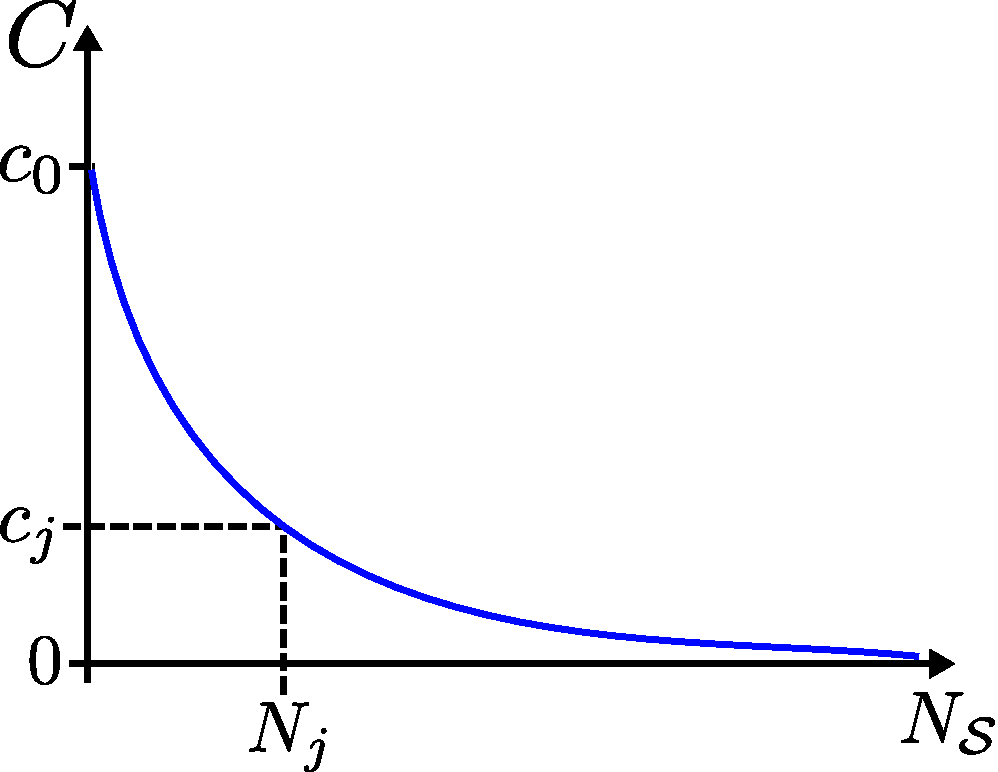
\includegraphics[width=0.7\columnwidth]{fig/complexity_per_cardinality.pdf}
% 	\caption{The complexity of a task $c_j$ (number of trial episodes) decreases exponentially with the number of learned tasks $|\mathcal{T}_j|=N_{j}$.}
% 	\label{fig:complexity_per_cardinality}
% \end{figure}
% % ---
% The assumption that there exist similarities among the different tasks in $\Tau$ implies that a new task $\tau_j \in \Tau$ can always benefit to a certain extent from the knowledge contained in $\mathcal{T}_j \subset \mathcal{T}$. This implies that the more tasks enter $\mathcal{T}_j$ (with $|\mathcal{T}_j| = N_j$), the more the similarity will increase, and the less knowledge will remain to be learned. Thus, according to \eqref{eq:scaled_complexity} the complexity scales down as a function of the number of learned tasks, as exemplified in Fig.~\ref{fig:complexity_per_cardinality}. Alternatively,
% % ---
% \begin{equation}\label{eq:knowledge_limit2}
%     \lim_{N_{j}\to N_{\mathcal{T}}} \bar{\sigma}_j(N_j) = 0 \implies \lim_{N_{j}\to N_{\mathcal{T}}} c_j = 0.
% \end{equation}

% \subsubsection{Isolated learning (Iso)} under this type of learning, a robot learns all the tasks in $\mathcal{T}$ one after another from scratch, disregarding the knowledge from all other learned tasks $\mathcal{T}_j$ when learning a new task. The energy required by the robot to learn all tasks in $\mathcal{T}$ is simply
% % ---
% \begin{equation}
%   E^{Iso}_{\mathcal{T}} = N_{\mathcal{T}} \cdot E_j = N_{\mathcal{T}} \cdot e_{0} \cdot c_{0} %N_{\mathcal{T}}\cdot P \cdot \Delta t \cdot \sum_{n=1}^{c_j} k_j^{(n)}.
% \end{equation}
% % ---
% % \begin{equation}
% %   E^{IL}_{\mathrm{tot} = e_o \sum_{i=1}^{n} c_0 = e_o \cdot n \cdot c_0.
% % \end{equation}

% Note that the task complexity $c_0$ remains unaltered. Furthermore, using batches of $m$ robots to learning $m$ tasks in parallel, needs $m\cdot E_j$ \unit[]{Joules}. Therefore, there are no energy reductions under this scheme.

% % ---------------------------------------------------------------------------------------------------
% \subsubsection{Transfer learning (T)}
% An idealization of the behavior described by \eqref{eq:knowledge_limit} can be modelled as a function that is exponentially decreasing with the number of already learned tasks:
% % ---
% \begin{equation}
%   \bar{\sigma}^{(T)}_j = e^{-\alpha  \cdot N_{j}} \in (0,1],
% \end{equation}
% % ---
% %\textcolor{red}{Plugging \eqref{eq:similarity_metric} into \eqref{eq:scaled_complexity}, it is easily seen that the complexity decreases exponentially, see Fig.~\ref{fig:complexity_per_cardinality}}.
% \hl{where $ 0<\alpha<<1$ models how effectively the knowledge contained in $\mathcal{T}_j$ is transferred to $\tau_j$.} With \eqref{eq:complexity_TL}, the scaling effect that transfer learning has on the task complexity is
% % ---
% \begin{equation}\label{eq:complexity_TL}
%   c^{(T)}_j = c_0 \cdot \bar{\sigma}^{(T)}_j = c_0 \cdot e^{-\alpha \cdot N_{j}}
% \end{equation}
% % ---
% If a batch of $m$ robots executes transfer learning; then, $ N_{j} = (j-1) \cdot m$. Therefore, the total energy for the batch of robots learning all the tasks in the batch is then,
% % ---
% \begin{equation}
%   E^{T}_j =    m \cdot c_0 \cdot e_0 \cdot \left.\bar{\sigma}^{(T)}_j \right\vert_{N_j = (j-1)\cdot m}.
% \end{equation}
% By extension, the total energy expenditure is
% \begin{align}\label{eq:itl_total_energy}
% \begin{split}
%   E^{T}_{\mathcal{T}} &= \sum^{{N_{\mathcal{T}}}/{m}}_{j=1} E^{T}_j \\
%   %& = m \cdot e_o  \cdot c_0 \sum^{{N_{\mathcal{T}}}/{m}}_{j=1} e^{- \alpha m (j-1) } \\
%   %& = m \cdot e_0 \cdot c_0 \cdot \left(\frac{1 - e^{ - \alpha N_{\mathcal{T}}}}{1 - e^{-\alpha m}}\right) 
% \end{split}
% \end{align}

% % ---------------------------------------------------------------------------------------------------
% \subsubsection{Incremental learning (I)}
% In incremental learning, the rate at which knowledge about a task is acquired depends on the number of learning episodes $n$; i.e. 
% % ---
% \begin{equation}
%   \bar{\sigma}^{(I)}_j = e^{-\beta \cdot (m-1) \cdot (c_0 - n)}  \in (0,1],
% \end{equation}
% % ---
% where, just like $\alpha$, $0<\beta<<1$ models the knowledge effectivity acquisition per episode. Consequently, the \emph{episodic complexity} is computed as
% % ---
% \begin{equation}
%   c^{(I)}_{j,n} = c^{(T)}_j \cdot {\bar{\sigma}^{(I)}_j} = c^{(T)}_j \cdot e^{-\beta \cdot (m-1) \cdot (c_0 - n)},
% \end{equation}
% % ---
% with $c^{(T)}_j = c_0$ if there is no transfer learning. Otherwise, \eqref{eq:complexity_TL} is used. After the compound effects of transfer and incremental learning, the scaled task complexity is the following:
% % ---
% \begin{equation}\label{eq:complexity_TIL}
% c^{(I)}_j = \left. c^{(I)}_{j,n}\right\vert_{n = c^{(T)}_j}
%           = c_0 \cdot \underbrace{\overbrace{\bar{\sigma}^{(T)}_j}^{transfer} \cdot \overbrace{\left.{\bar{\sigma}^{(I)}_j}\right\vert_{n = c^{(T)}_j}}^{incremental}}_{\text{remaining knowledge}},
% \end{equation}
% % ---
% Fig.~\ref{fig:complexity_TIL} depicts the exponentially decreasing complexity for transfer learning and for the incremental wit transfer learning.
% % ---
% \begin{figure}[!t]
% 	\centering
% 	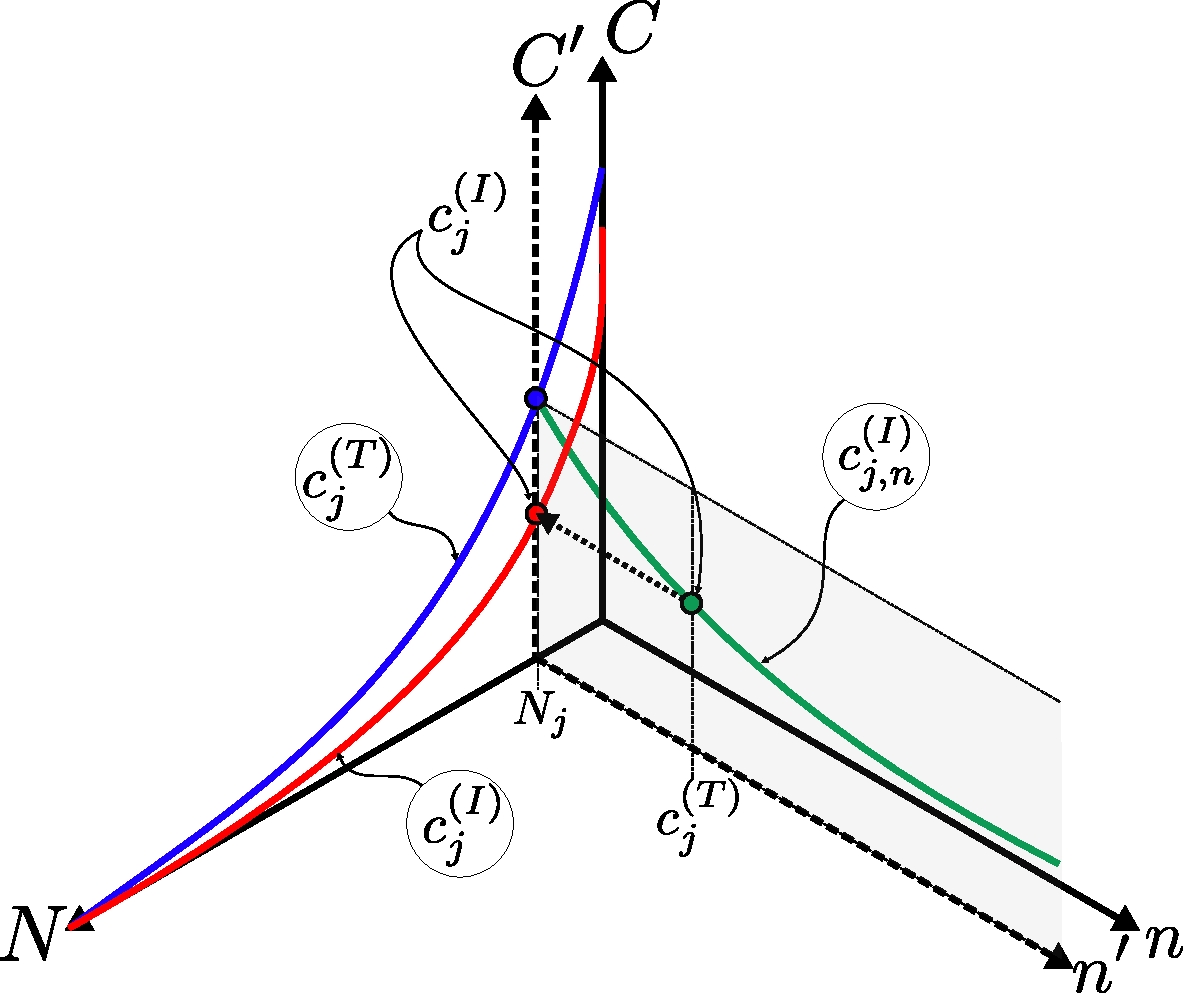
\includegraphics[width=0.99\columnwidth]{fig/concept_TIL.pdf}
% 	\caption{The reduction of task complexity in incremental-transfer learning.}
% 	\label{fig:complexity_TIL}
% \end{figure}
% % ---

% To compute the energy spent by a batch of $m$ robots using transfer and incremental learning, we plug \eqref{eq:complexity_TIL} into \eqref{eq:energy_per_task}, obtaining,
% % ---
% \begin{align}\label{eq:itl_energy_per_task}
% \begin{split}
%     E^{IT}_j &= m \cdot e_0 \cdot c^{(I)}_j\\
%     &= m \cdot c_0 \cdot e_0 \cdot \left.\bar{\sigma}^{(T)}_j \right\vert_{N_j = (j-1)\cdot m} \cdot \left.{\bar{\sigma}^{(I)}_j}\right\vert_{n = c^{(T)}_j}.
%     %&= m \cdot e_0 \cdot c^{(T)}_j \cdot e^{-\beta \cdot (m-1) \cdot c^{(T)}_j}\\
%     %&= m \cdot e_0 \cdot c_0 \cdot e^{-\alpha \cdot m \cdot (j-1)} \cdot e^{-\beta \cdot (m-1) \cdot \left(c_0 \cdot e^{-\alpha \cdot m \cdot (j-1)}\right)}\\
% \end{split}    
% \end{align}
% % ---
% Respectively, the total energy for a batch of robots learning all tasks is then
% % ---
% \begin{align}\label{eq:itl_total_energy}
%   E^{IT}_{\mathcal{T}} &= \sum^{{N_{\mathcal{T}}}/{m}}_{j=1} E^{IT}_j
% \end{align}

% % ---------------------------------------------------------------------------------------------------
% \subsubsection{Collective learning (C)}
% Here, each robot has access to the knowledge previously acquired by all the $m$ robots in the collective, as well as to the knowledge being concurrently acquired by itself and all the other $m-1$ robots learning $m-1$ new tasks in every episode, and also the knowledge that is acquired per iteration. %Therefore, under the collective learning paradigm, the similarity metric defined in \eqref{eq:similarity_metric} no longer depends only on the already acquired knowledge, but also on the knowledge being concurrently being learned by the robots in the collective learning $m$ different tasks. 
% Thus, the similarity metric is now modelled as
% \begin{equation}
%   \bar{\sigma}^{(C)}_j = e^{-\gamma \cdot (m-1) \cdot \overbrace{k \cdot (c_0 - n)}^{iterations}}  \in (0,1],
% \end{equation}
% % ---
% where $0<\gamma<<1$ models the knowledge acquisition effectivity \textbf{per iteration} and $k$ denotes the fixed number of iterations per episode $n$ (Assumption~\ref{assumption:time}). Consequently, the \emph{iteration complexity} is computed as
% % ---
% \begin{equation}
%   c^{(C)}_{j,n} = c^{(I)}_j \cdot {\bar{\sigma}^{(C)}_j} = c^{(I)}_j \cdot e^{-\gamma \cdot (m-1) \cdot k \cdot (c_0 - n)},
% \end{equation}
% % ---
% After the compound effects of transfer, incremental, and collective learning, the scaled task complexity is
% % ---
% \begin{align}\label{eq:complexity_CL}
% c^{(C)}_j = \left. c^{(C)}_{j,n}\right\vert_{n=c^{(I)}_j}
%           = c_0 \cdot \overbrace{\bar{\sigma}^{(T)}_j}^{transfer} \cdot \underbrace{\left.{\bar{\sigma}^{(I)}_j}\right\vert_{n = c^{(T)}_j}}_{incremental}\cdot \overbrace{\left.\bar{\sigma}^{(C)}_j\right\vert_{n=c^{(I)}_j}}^{collective}
%     %c^{(I)}_j &=  \left. c^{(T)}_j \cdot e^{-\beta \cdot (m-1) \cdot n} \right\vert_{n = c^{(T)}_j}
% \end{align}
% % ---
% Fig.~\ref{fig:complexity_CL} shows how the task complexity is reduced under collective learning.
% % ---
% \begin{figure}[!t]
% 	\centering
% 	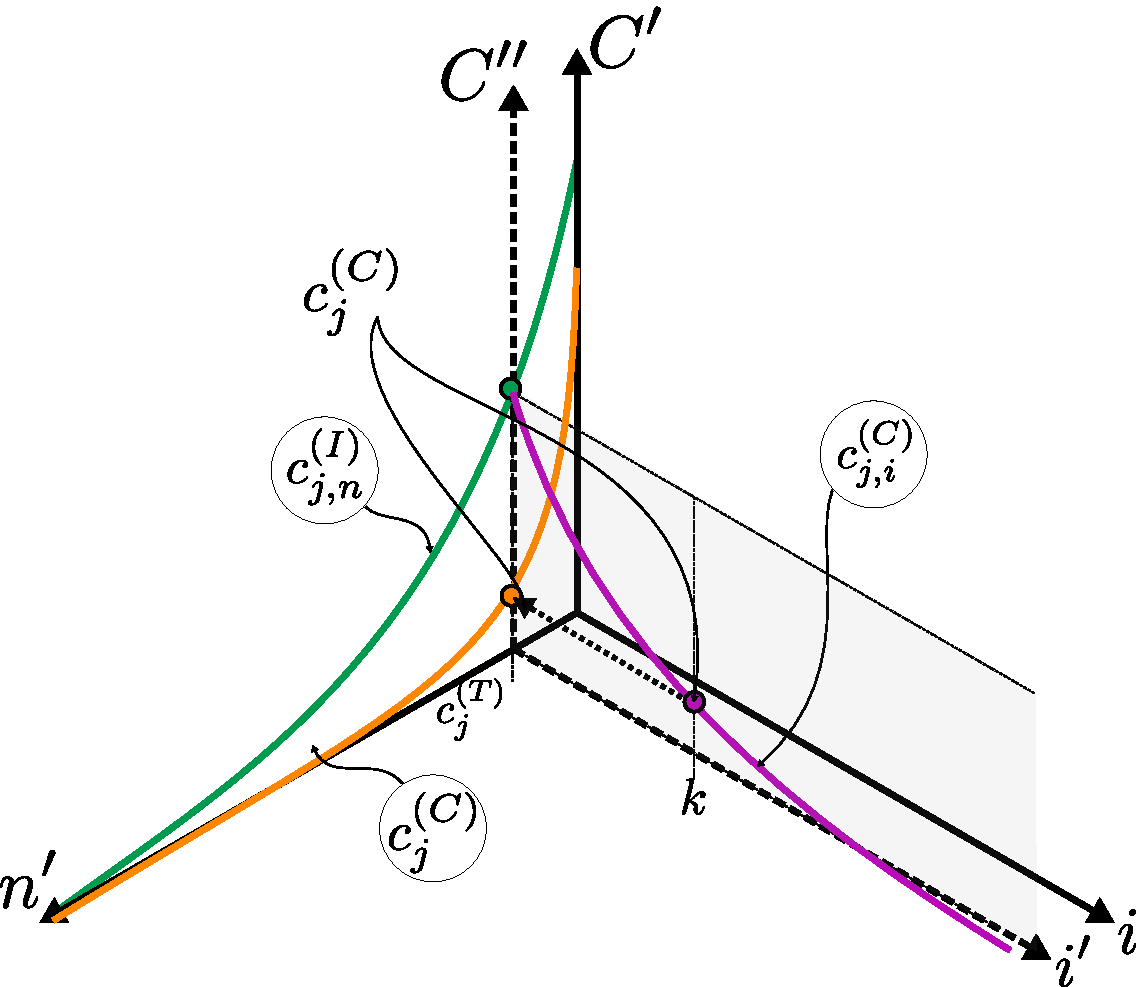
\includegraphics[width=0.99\columnwidth]{fig/concept_CL.pdf}
% 	\caption{The reduction of task complexity using collective learning.}
% 	\label{fig:complexity_CL}
% \end{figure}
% % ---
% To compute the energy spent by a batch of $m$ robots using transfer, incremental, and collective learning, we plug \eqref{eq:complexity_CL} into \eqref{eq:energy_per_task}, obtaining,
% % ---
% \begin{align}\label{eq:cl_energy_per_task}
% \begin{split}
%     E^{C}_j &= m \cdot e_0 \cdot c^{(C)}_j\\
%     &= m \cdot c_0 \cdot e_0 \cdot \left.\bar{\sigma}^{(T)}_j \right\vert_{N_j = (j-1)\cdot m} \cdot \left.{\bar{\sigma}^{(I)}_j}\right\vert_{n = c^{(T)}_j} \cdot \left.\bar{\sigma}^{(C)}_j\right\vert_{n=c^{(I)}_j}.
% \end{split}    
% \end{align}
% % ---
% Respectively, the total energy for a single robot learning all tasks is then
% % ---
% \begin{align}\label{eq:cl_total_energy}
%   E^{C}_{\mathcal{T}} &= \sum^{{N_{\mathcal{T}}}/{m}}_{j=1} E^{C}_j
% \end{align}

% % ---------------------------------------------------------------------------------------------------
% \subsubsection{Comparison of the different learning complexities}
% Ultimately, depending on the values for the constants $\alpha$, $\beta$, and $\gamma$
% % ---
% \begin{equation}
% c_j =
%     \begin{cases} 
%       c_0 & \alpha=\beta=\gamma =0 \\
%       c^{(T)}_j & \alpha\neq 0, \beta=\gamma =0 \\
%       c^{(I)}_j & \alpha\neq 0, \beta \neq 0, \gamma =0 \\
%       c^{(C)}_j & \alpha\neq 0, \beta \neq 0, \gamma \neq 0 
%   \end{cases}
% \end{equation}
% % ---
% Finally, the complexity demand per task for the different learning schemes is shown in Fig.~\ref{fig:learning_schemes}.
% % ---
% \begin{figure}[!t]
% 	\centering
% 	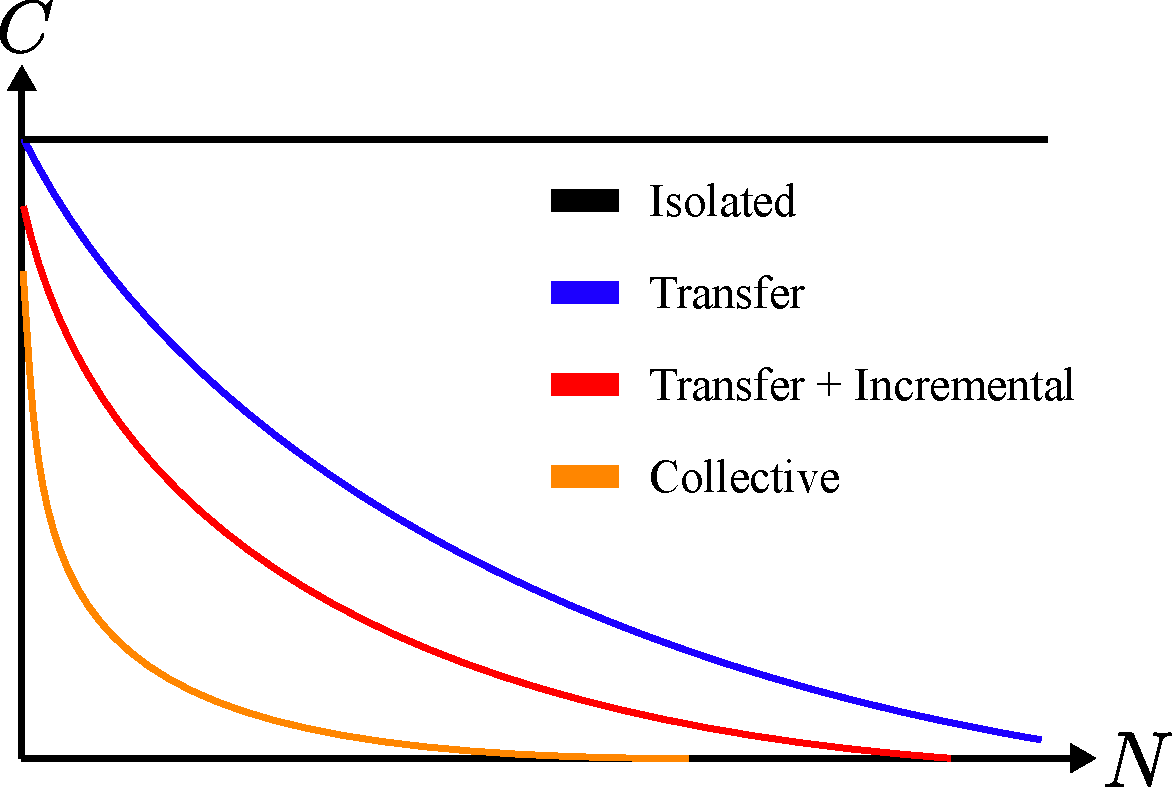
\includegraphics[width=1\columnwidth]{fig/complexity_per_tasks.pdf}
% 	\caption{Reduction of task complexity for the different learning schemes.}
% 	\label{fig:learning_schemes}
% \end{figure}
